\documentclass[a4paper]{article}


%%% ENCODING, FONT & LOCALIZATION
\usepackage[utf8]{inputenc} % use unicode input-encoding (allows unicode characters in the .tex files, default: Asci)
\usepackage{lmodern} % vectorized version of the "computer modern" font (default) (https://tex.stackexchange.com/q/1390/148164, https://tex.stackexchange.com/q/147194/148164)
\usepackage[ngerman, english]{babel} %% last language is main
%\shorthandoff{"} %babel breaks tikz-cd otherwise (activate if used)
\usepackage{csquotes} %% biblatex wants csquotes (localized quotes) if babel is present

%%% GENERAL IMPROVEMENTS
\usepackage[unicode, hidelinks]{hyperref} %% clickable links
\usepackage{enumitem} %% better (customizable) enumerations (e.g. \begin{enumerate}[label=(\roman*)])


%%% STYLING
% \setlength{\parindent}{0em} % No indentation for new paragraphs
\usepackage{emptypage} % removes page numbers on empty pages
% \makeatletter \@twosidefalse \makeatother
\usepackage{xcolor}


%%% GRAPHICS & PLOTS

% \usepackage{graphicx} % enable pictures
\usepackage{wrapfig} % text wrapping around figures
% \usepackage{tikz, tikz-cd, pgfplots} % plots and sketches
% \pgfplotsset{compat=1.16}

%%% CODE
\usepackage[ruled,linesnumbered]{algorithm2e}

% fix algomathdisplay (see: https://tex.stackexchange.com/a/611426/148164)
\makeatletter
\renewenvironment{algomathdisplay}
 {\[}
 {\@endalgocfline\vspace{-\baselineskip}\]{\DontPrintSemicolon\;}}
\makeatother
%%% MATH
\usepackage{mathtools} % fixes some things from amsmath and adds some new features
\usepackage{amsthm, amssymb} % amsthm -> proof env, amssymb -> additional symbols
\usepackage{aligned-overset} % https://tex.stackexchange.com/questions/257529/overset-and-align-environment-how-to-get-correct-alignment
%% usage: \overset{something}&{=}

%%% Special Symbols
% \usepackage{bbm} % blackboard numbers: usage \mathbbm{1} (amssymb \mathbb{1} looks bad)
% \usepackage{cancel} % strike through equation parts to indicate they cancel out
% %% contradiction symbol
% \usepackage{wasysym} % lightning symbol
% \newcommand*{\contradiction}[1][]{\quad\text{{\LARGE\lightning} #1}\ }

%%% EDITING (Annotations, TODO, etc.) 
\usepackage[draft]{fixme} %final removes annotations %draft includes annotations
\fxsetup{theme=color}
%%\fxnote{some note} ,\fxwarning{}, \fxerror{}, \fxfatal{} <- does not allow [final] to compile

%%% BIBLIOGRAPHY
\usepackage[style=alphabetic, backend=biber, seconds=true, date=iso, urldate=iso, maxcitenames=2]{biblatex}
\addbibresource{references.bib}

%% AMS Theorem Environments
\theoremstyle{plain}% default
\newtheorem{prop}{Proposition}[section]
\newtheorem{lemma}[prop]{Lemma}
\newtheorem{corollary}[prop]{Corollary}
\newtheorem{theorem}[prop]{Theorem}

\theoremstyle{definition}
\newtheorem{definition}[prop]{Definition}
\newtheorem{example}[prop]{Example}
\newtheorem*{example*}{Example}
\newtheorem{assumption}[prop]{Assumption}

\theoremstyle{remark}
\newtheorem{remark}[prop]{Remark}

%%

\newcommand{\E}{\mathbb{E}}
\renewcommand{\Pr}{\mathbb{P}}
\DeclareMathOperator{\sgn}{sgn}
\DeclareMathOperator*{\argmax}{argmax}
\DeclareMathOperator{\diag}{diag}
\newcommand{\identity}{\mathbb{I}}
\DeclareMathOperator{\conv}{Conv}
\DeclareMathOperator{\pf}{PF}
\DeclareMathOperator{\wtb}{wtb}
\DeclareMathOperator{\wtp}{wtp}
\newcommand{\ind}{\mathbbm{1}}

\newcommand*{\real}{\mathbb{R}}
\newcommand*{\nat}{\mathbb{N}}
\newcommand*{\dims}{d}


\title{General Equilibrium}
\author{Felix Benning}

\begin{document}
	\maketitle 

	\begin{abstract}
	Lorem Ipsum etc.	
\end{abstract}
	\section{Hermits}

Let \(X_i = X_i(L_i)\) be the set of possible production vectors of person \(i\)
under labour constraint \(L_i\).

\begin{figure}
	\centering
	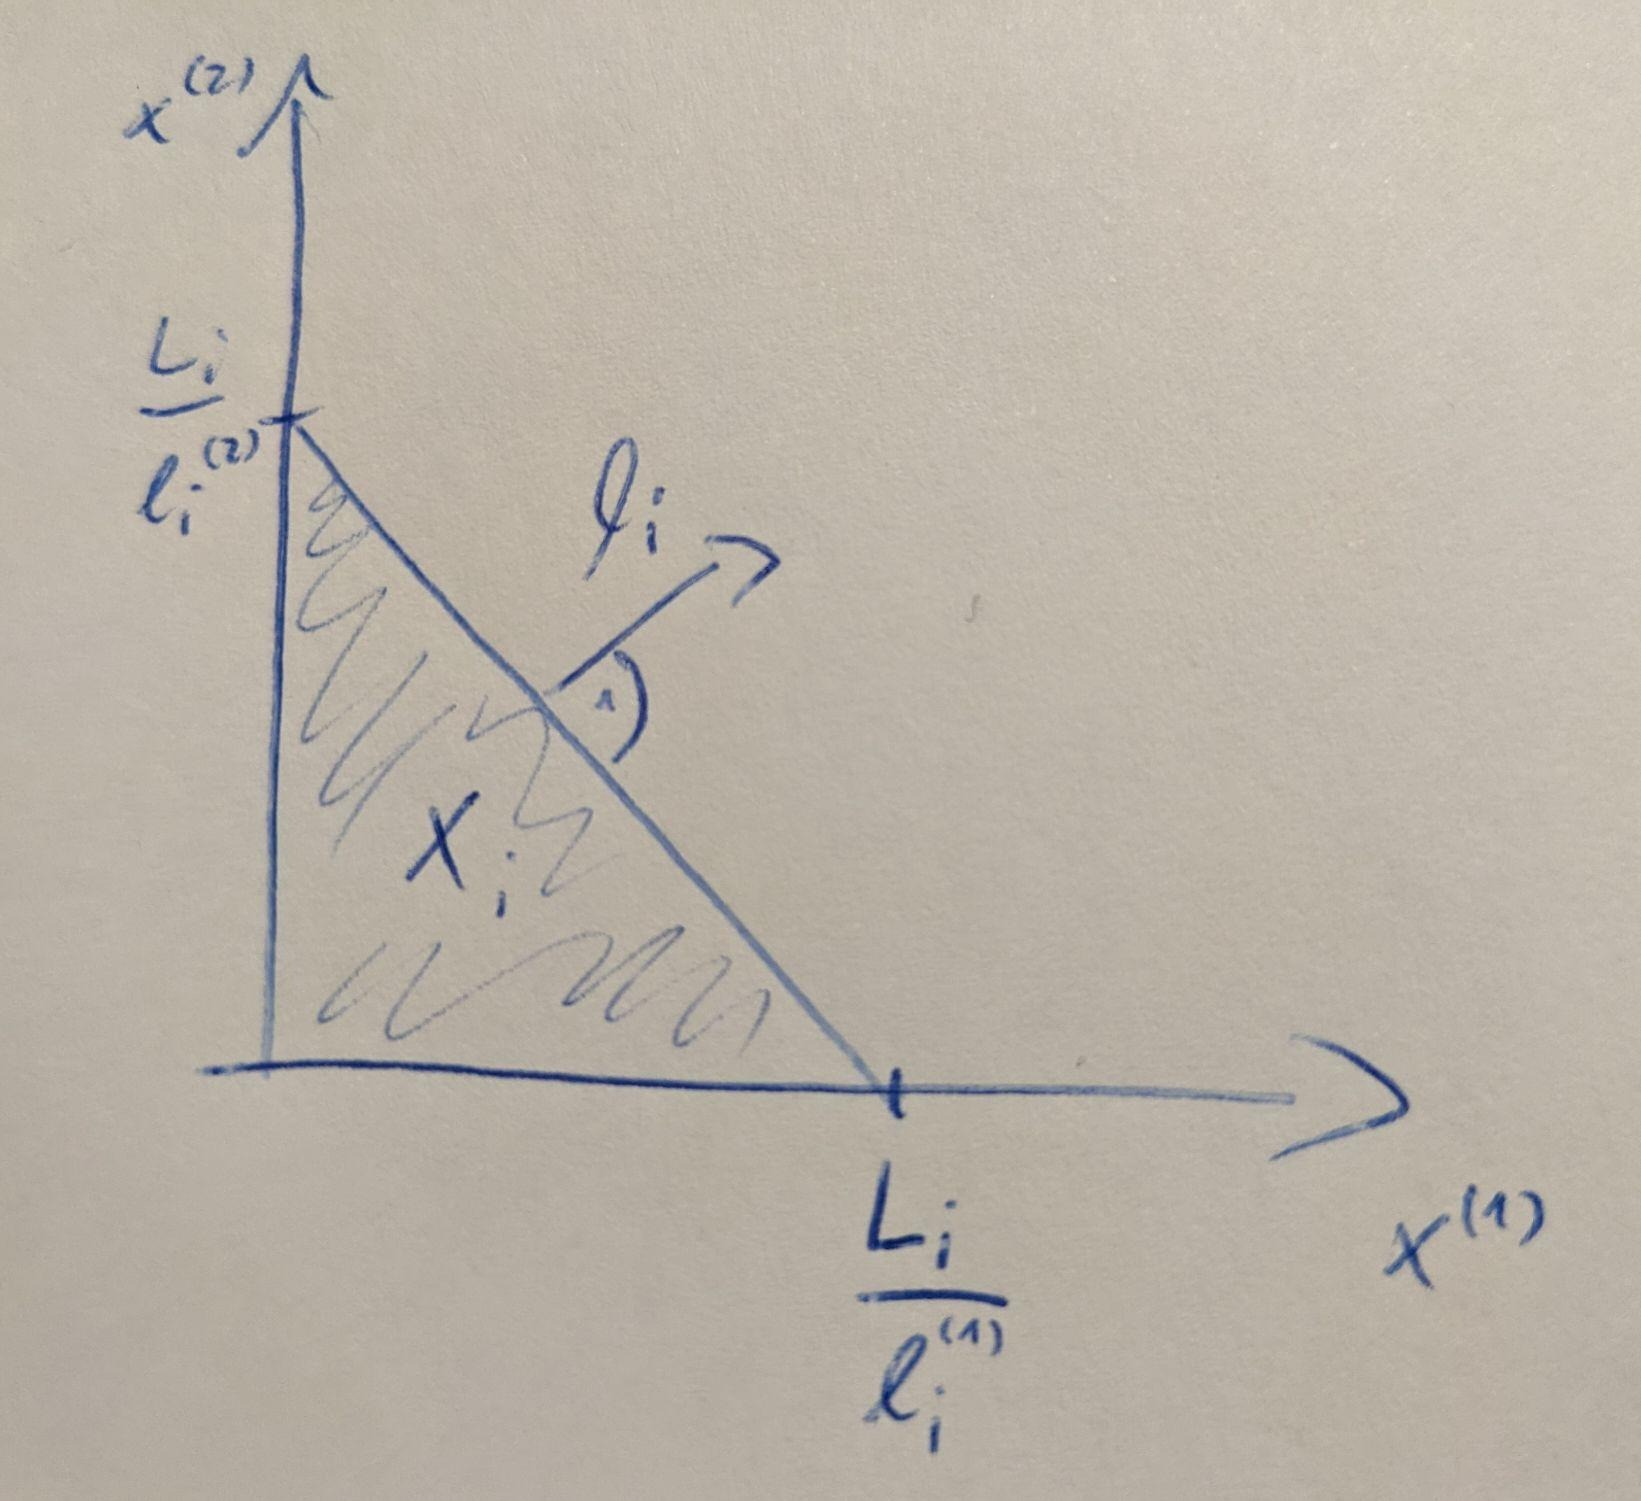
\includegraphics[width=0.46\textwidth]{images/pure-variable-cost.jpeg}
	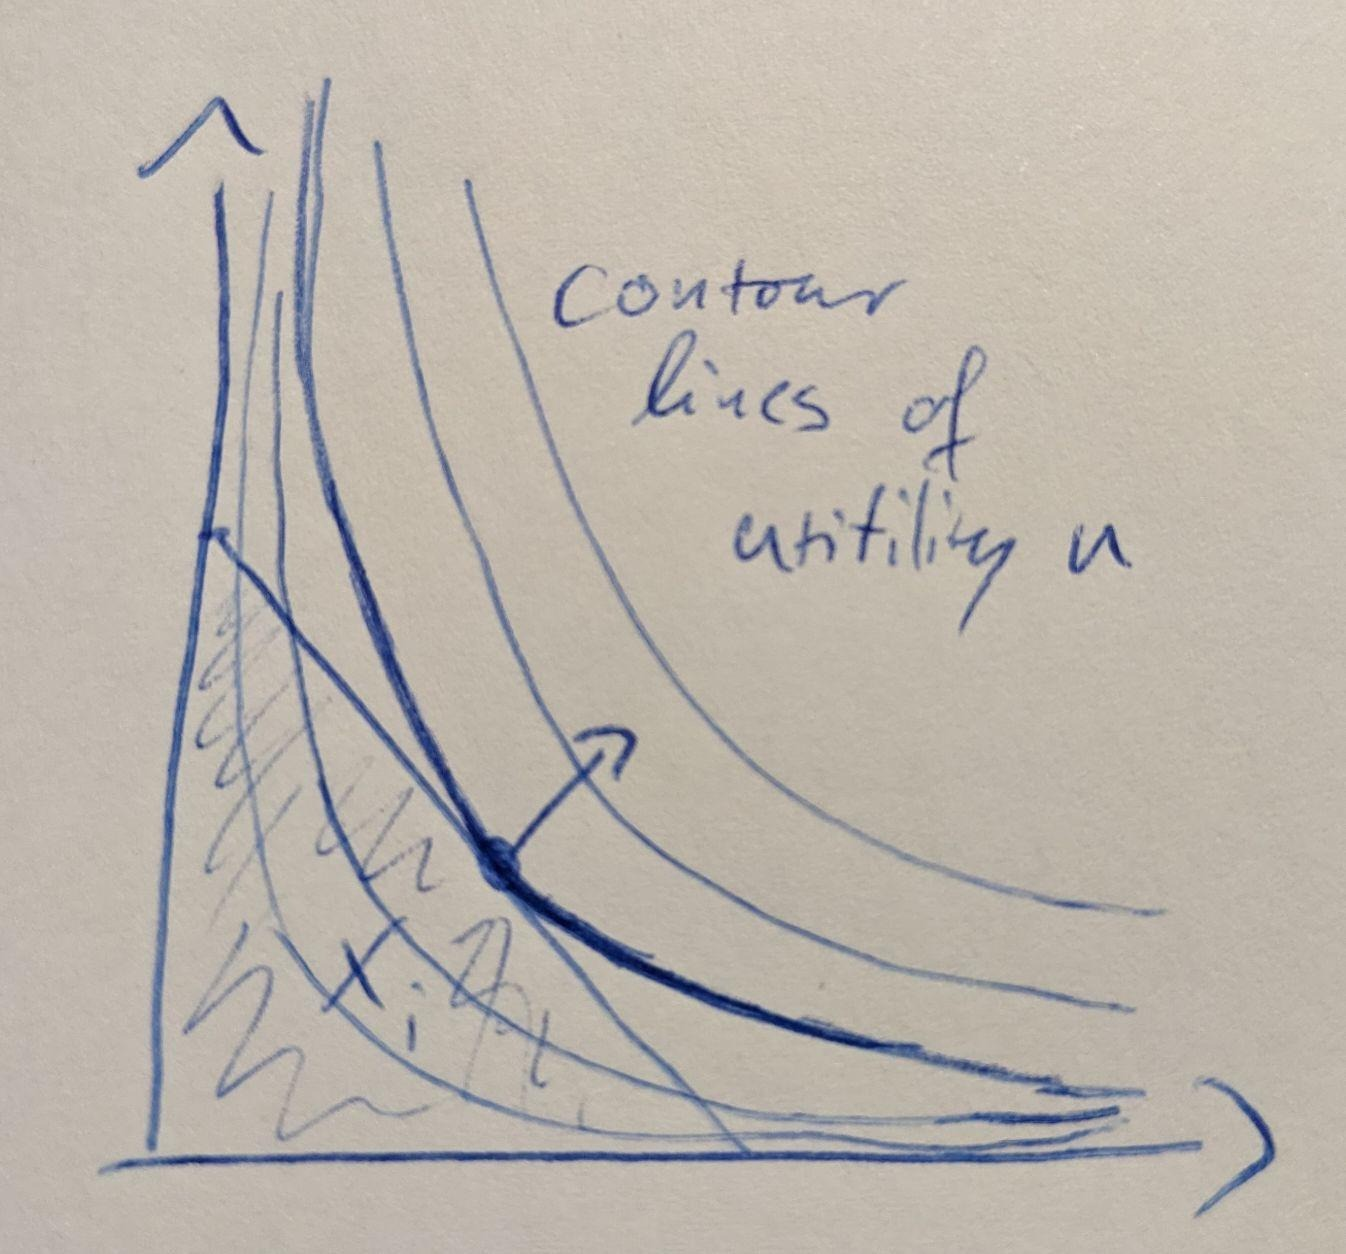
\includegraphics[width=0.45\textwidth]{images/hermit-decision-pure-variable.jpeg}
	\caption{
		Pure Variable Cost \(X_i\) on the left. The hermits decision problem
		on the right.
	}
\end{figure}
\begin{example*}[Pure Variable Costs]
	One important special case is
	\[
		X_i = \{ x \in \real_{\ge 0}^\dims: \langle x, l_i \rangle \le L_i \}.
	\]
	Here \(l_i^{(j)}\ge0\) is the labour time required by person \(i\) to produce one
	unit of good \(j\). Therefore the total time spent to produce quantity
	\(x^{(j)}\) of good \(j\) is \(x^{(j)}l_i^{(j)}\). Summing over all goods
	results in the total time requirement
	\[
		L_i(x) = \sum_{j=1}^\dims x^{(j)}l_i^{(j)} = \langle x, l_i\rangle,
	\]
	which obviously needs to be smaller than our time constraint \(L_i\).

	One could easily model exhaustion with \(L_i(x) = g(\langle x, l_i\rangle)\)
	for some strictly monotonously increasing function \(g\). You could also
	view \(L_i(x)\) more generally as the discomfort of labour instead of merely
	the time required, to generalize to tasks which take longer but are more
	enjoyable and vice versa.
\end{example*}

A hermit therefore faces the utility function maximization problem
\[
	\max_{L_i, x} u(\overbrace{1-L_i}^{\text{free time}}, x)
	\quad\text{subject to}\quad x\in X_i(L_i).
\]
going back to our special case, this has a very intuitive interpretation.


\begin{example*}[Pure Variable Costs]
	In the pure variable cost case, the hermits decision problem simplifies to
	\[
		\max_{x} u(\overbrace{1-L_i(x)}^{\text{free time}}, x).
	\]
	So denoting the partial derivative with regard to free time as \(u_f\) and
	the gradient vector with regard to \(x\) as \(u_x\), the first order
	condition for maximization requires
	\[
		0\overset!=\frac{du}{dx}
		= u_x - \nabla L_i(x) u_f
		= u_f \Bigl[
			\underbrace{\frac{u_x}{u_f}}_{\mathclap{\text{willingness to work (wtw)}}}
		- \overbrace{\nabla L_i(x)}^{\mathclap{\text{natural prices}}}
		\Bigr],
	\]
	where we can assume the marginal utility of more free time \(u_f\) to be
	positive. The natural prices are simply {\color{lightgray} a multiple of}
	\(l_i\)
	\[
		\nabla L_i(x) = {\color{lightgray} g'(\langle x, l_i\rangle) }l_i.
	\]
	In other words: the price of good \(j\), is the {\color{lightgray} marginal}
	time required to produce \(j\). And without exhaustion this is simply
	\(l^{(j)}_i\). If the willingness to work for good \(j\) is smaller than
	its price, then our gradient is negative in this direction. Meaning that
	a reduction of \(x^{(j)}\) would increase our utility. If \(\text{wtw}^{(j)}\) is
	greater than the price of \(j\), an increase of \(x^{(j)}\) increases utility.
\end{example*}
	\section{Aggregate Production Capabilities}

The total production capabilities \eqref{eq: tpc} of a society of \(n\) people, is given by the
Minkowski sum of individual production capabilities
\begin{equation}
	\label{eq: tpc}\tag{TPC}
	X = \{ x_1 + \dots + x_n : x_i \in X_i\} = \sum_{i=1}^n X_i
\end{equation}

If we split the spoils of production equally between everyone, then the set of
possible consumption vectors is given by the average production capability
\begin{equation}
	\label{eq: apc}\tag{APC}
	\bar{X}_n = \tfrac1n X = \{\tfrac{x}n : x\in X\}.
\end{equation}

In a society of identical clones, this is what we would expect to happen.

\begin{lemma}[Clone Production Capabilities]
	In a society of clones, we have \(X_1=\dots = X_n\). Then we observe:
	\begin{enumerate}
		\item In general we have \(X_1\subseteq \bar{X}_n\).
		\item If we assume that \(X_1\) is convex, then
		\[
			\bar{X}_n = X_1
		\]
		\item Using only the \ref{eq: lower layer} property of \(X_1\), we get
		\[
			\bar{X}_n \to \conv(X_1),
		\]
		where \(\conv(M)\) is the convex hull\footnote{
			The convex hull is defined as the set of all convex combinations
			\[
				\conv(M)= \Bigl\{\sum_{i=1}^m \lambda_i x_i : m\in\nat,\ x_i \in M,\ \lambda_i\in[0,1],\ \sum_{i=1}\lambda_i =1\Bigr\}
			\]
		} of the set \(M\) and we define
		convergence of sets as follows: \(M_n\) converges to \(M\), if

		\begin{enumerate}
			\item\label{set-conv: seq} For all \(x\in M\) exists a sequence
			\(x_n\in M_n\) with \(x_n\to x\).

			\item\label{set-conv: incl} For all \(x\) in the interior \(M^\circ\)
			of \(M\), exists \(n_0\in\nat\) such that \(x\in M_n\) for all \(n\ge
			n_0\).
		\end{enumerate}
		The \ref{eq: lower layer} property is only needed for \ref{set-conv:
		incl}.
	\end{enumerate}
\end{lemma}

\begin{proof}
\begin{enumerate}
	\item For \(X_1 \subseteq \bar{X}_n\), we take \(x\in X_1\) and
	observe that if we pick 
	\[
		x_1=\dots=x_n=x
	\]
	in the Minkowski sum we obtain \(n x \in X\). So we have
	\(x\in\bar{X}_n\).
	

	\item
	Equality in the convex case is almost trivial as well. Let \(x\in
	\bar{X}_n\), then there exist \(x_1,\dots,x_n \in X_1\) such that \[
		x = \frac1n \sum_{i=1}^n x_i = \sum_{i=1}^n \frac1n x_i
		\overset{\text{convex}}\in X_1.
	\]

	\item
	\begin{enumerate}
		\item Pick \(x\in \conv(X_1)\). Since it is in the convex hull,
		there exist \(\lambda_1,\dots,\lambda_m\) summing to unity, \(x_i\in X_1\)
		with
		\[
			x = \sum_{i=1}^m \lambda_i x_i.
		\]
		We set the number of clones producing \(x_i\) to the largest integer smaller
		\(n\lambda_i\)
		\[
			k_i^{(n)} := \lfloor n\lambda_i \rfloor.
		\]
		This is possible due to	
		\[
			\sum_{i=1}^m k_i^{(n)} \le n \sum_{i=1} \lambda_i = n.
		\]
		This results in
		\[
			x^{(n)}:= \frac1n\sum_{i=1}^m k_i x_i \in \bar{X}_n.
		\]
		Due to \(\frac{k_i^{(n)}}{n}\to \lambda_i\), we can conclude \(x^{(n)}\to
		x\).
		
		\item
		Pick any \(x=(x^{(1)},\dots,x^{(\dims)})\in\conv(X_1)^\circ\). Since it is
		in the interior, there exists \(\epsilon>0\) such that
		\[
			x_{+\epsilon}
			:= (x^{(1)}+\epsilon, \dots, x^{(\dims)}+\epsilon) \in \conv(X_1)^\circ.
		\]
		By \ref{set-conv: seq} we know there exists a sequence
		\(x_n\in\bar{X}_n\) with \(x_n\to x_{+\epsilon}\), and therefore there exists
		\(n_0\in\nat\) such that for all \(n\ge n_0\), \(x_n\) is included in the
		\(\epsilon\) ball induced by the sup-norm around \(x_{+\epsilon}\). But this
		implies \(x^{(i)} \le x^{(i)}_n\) for all \(n\ge n_0\). As the \ref{eq: lower
		layer} property easily translates\footnote{
			the lower layer property essentially allows us to throw away surplus. It
			is intuitive that we can do that with the total output as well. To show
			this mathematically we only need to distribute this ``throwing away''
			action among the producers of the product we want to throw away.
		} to the
		Minkowski sum and the average production capabilities \(\bar{X}_n\), we
		conclude \(x\in\bar{X}_n\) for all \(n\ge n_0\).
		\qedhere
	\end{enumerate}
\end{enumerate}
\end{proof}

In general, the production sets \(X_i\) are obviously not equal. But assuming
they are drawn from some sort of probability distribution, it seems plausible
that \(\bar{X}_n\) would still converge to a convex set. But defining a
probability distribution over the sets with the \ref{eq: lower layer} property,
is not trivial to do. Later we will consider the special case of an
extended pure variable cost case (with setup costs), where the costs are random
variables.\fxnote{add reference}
	\section{Motivating Prices}

While \(\bar{X}_n\) is great to build intuition about societies of people, all
its elements are \(n\)-th portions of some total production vector \(x\in X\).
This suggests that everyone would consume the exact same things. And while
clones are great and all, that is not what we are interested in. So how could
multiple people share the goods they produced, without necessarily consuming the
exact same things? 

To satisfy the ``Pluralism in Economics'' crowd, let us avoid
the term ownership for now. We simply observe that some people will produce
things and not necessarily the same people will consume\footnote{
	You can turn a product you can use \(m\) times (before it breaks down)
	without loss of generality into a consumable, by considering these \(m\) uses
	to be individual products. So a person does not ``have'' a chair, but rather
	the \(i\)-th usage of said chair. With this trick in mind, all products are
	consumable.
} the products.
No matter how you organize a society, from an individual perspective, there
are going to be goods the individual \(i\) produces \(S_i\in\real^\dims\) and
goods the individual consumes \(D_i\in\real^\dims\). And fundamentally a
society cannot consume more than is produced (and probably does not want to
produce more than necessary), so we need
\[
	S = \sum_{i=1}^n S_i = \sum_{i=1}^n D_i = D.
\]
The big question is: how can we ensure this? We also want everyone to
voluntarily participate in society. And people are going to stop doing so, if
they feel ripped off as they contribute much more than they get back.
Unfortunately it is difficult to compare the size of two vectors \(S_i\) and
\(D_i\) of uncomparable products. Of course we could enforce \(S_i=D_i\), but
then we are back to hermits, since everyone is using only what they produce.

To make the products comparable again, we could measure them by the time it took
to produce them. In other words the effort required for them. But recall that
the time needed to produce good \(j\), \(l_i^{(j)}\), might be different for
every person \(i\). Additionally this time is private information of person
\(i\). Especially if we generalize it to be a discomfort measure instead of
strictly time.


\begin{example}[Definitely not Capitalism]
	\label{ex: Definitely not Capitalism}
	Let us try to build a communist utopia, without money and ownership.  For
	this assume that the person which produces good \(j\) jots down their
	subjective cost of production \(l_i^{(j)}\) and tags the product with it and
	puts it into a communal holding space. Additionally they add the cost to
	their ``work-time'' tally.  Whenever someone wants to consume the product,
	they add the cost to their ``consumption-time'' tally, and take the product
	from communal holding space.  Everyone makes sure that their ``work-time''
	tally is comparable to their ``consumption-time''. We have tags, because
	people are bad at estimating how much effort is behind the products they
	consume.

	Does this sound like a utopia? Great!
	We can simplify the two tallies into one, because we only want to make
	sure that the difference is approximately zero. So we might as well add
	``work-time'' and subtract ``consumption-time'' from the get go. We also do not
	need to know how the current tally came to be, so we only need to keep track
	of the running total. This total is going to fluctuate around zero. When it
	is positive, you have worked more for society than you have consumed. And
	vice versa when it is negative.

	Now consider the life of a single product. When it is consumed, the cost was
	added to the tally of the producer and subtracted from the consumer. If you
	had chips to represent the tally, then they would have been simply passed from
	the consumer to the producer. Oh, wait! That's money! People are trading goods
	for money!

	Although right now, tallies can be negative and we do not have negative
	chips/money. This is a problem if you start out with everyone at zero. Because
	nobody can go below that. Or can they? If Alice signs a piece of paper saying
	she owes \(x\) amount of work-time, then she can pass that for a product that
	costs \(x\). The person receiving this note could then pass this note on to
	pay for something too. And if everyone trusts Alice, this is going to go
	swimmingly. So in principle anyone can create money. Money is just the debt
	of someone. The difficulty is creating debt which is widely accepted.

	The balance on a bill splitting app is money (in your friends circle), a coupon
	is money (scammers like to be paid in it), etc. But the money which is most
	widely accepted, is the money issued by a trusted government. Because money is
	debt, so the question whether you accept is, is whether you trust the debtor.
\end{example}
\begin{remark}
	Example~\ref{ex: Definitely not Capitalism} is supposed to show how difficult
	it is to come up with a system which balances production and consumption,
	which is not mathematically equivalent to a market economy. And while the
	initially proposed tally system might be mathematically equivalent, it is
	much less robust and efficient in reality. Because you need to \emph{trust}
	people to update their tallies accurately, \emph{trust} that they make sure
	they don't go too far into the negative, and you need to travel to a
	communal holding space instead of conducting exchanges \emph{decentrally}.
\end{remark}

\subsection{Prices as a Measure of Effort}

In the hopes that we justified ownership, trade and prices sufficiently, let us
consider this in more detail. We have suggested using \(l^{(j)}_i\) as prices
(i.e. the effort required for production).  This implies that one good \(j\) has
different prices, depending on the producer \(i\). Since we assume that there
are no quality differences, people will obviously buy the cheaper products
first. Let \(p_j\) be the largest price for which good \(j\) is ever sold.
Potential producers \(i\) with \(l^{(j)}_i > p_j\) refrain from producing good
\(j\) and focus their attention on other products.

The producers with \(l^{(j)}_i < p_j\) now see, that they could have sold their
goods for more. And since the cost of production \(l^{(j)}_i\) is private
information, they will likely claim that this cost went up a little next time.
I.e. in the long run, only one prices \(p_j\) per good \(j\) is stable.
\begin{quotation}
\noindent Price \(p_j\) roughly measures the effort required to produce \(j\) by
the least efficient producer of \(j\).
\end{quotation}

The question remains: What is the right price? Should we average the
\(l^{(j)}_i\) somehow?

Since we are implicitly selecting the cutoff of who is going to produce \(j\) by
setting \(p_j\) and we want to ensure supply to be equal to demand \(S=D\), it
turns out we have very little choice when it comes to prices anyway. Let us see
what happens for a fixed price vector. We want \(S=D\). This obviously implies
\begin{equation}
	\label{eq: supply gdp = demand gdp}
	0 =\langle S-D,p\rangle =  \sum_{i=1}^n \langle S_i - D_i, p\rangle
\end{equation}
A market based system on the other hand ensures
\[
	0 = \langle S_i - D_i, p\rangle
	= \underbrace{\langle S_i, p\rangle}_{\text{income}}
	- \underbrace{\langle D_i,p\rangle}_{\text{expenses}}
\]
which is more than sufficient for the sums in Equation~\eqref{eq: supply gdp =
demand gdp} to be equal, but not sufficient for \(S=D\). In fact, it only
ensures that the price is orthogonal to the demand/supply mismatch \(S-D\).
If there are \(d\) products, that leaves a \(d-1\) hyperplane.

But as we will see, there are some price vectors, which do ensure \(S=D\).
We call these economic equilibria.

\subsection{Money Supply and Price Stability}
\label{subsec: money supply and price stability}

Since everyone simply ensures that their income is equal to their expenses, i.e.
that \(S_i - D_i\) is orthogonal to \(p\)
\[
	0 = \langle S_i - D_i, p\rangle,
\]
scaling of \(p\) has no effect on anyone's decision. So if \(p^*\) is an
economic equilibrium, so is \(cp^*\) for every \(c\in \real_{>0}\). So it
appears we have a surplus of one degree of freedom for \(p\). As it will turn
out, we lose that degree of freedom to the money supply.
The gross domestic product (GDP) is defined to be the sum of all transactions.
One way to calculate it, is to sum up all sales made by each individual
\[
	\text{GDP} = \sum_{i=1}^n \langle p, S_i\rangle = \langle p, S\rangle.
\]
If our economy runs on money (instead of some tally) on the other hand, there
is typically a fixed supply \(M\). If people receive payment at the start of
the month (wages) and spend it during the month, then the entire money supply
will be used once per month. This is of course a bit too simplistic, but the
point here is, that the money velocity \(V\) (i.e. the amount of times the same
coin changes hands per month or other time unit) is typically externally fixed.
But if we want to sum all transactions, and we know the size of the money supply
and also its cycle velocity, then we already know the total size of all
transactions:
\[
	\text{GDP} = MV.
\]
So it is necessarily true, that 
\begin{equation}
	\label{eq: nominal GDP equation}
	\langle p, S\rangle = MV.	
\end{equation}
If the society now manages to produce \(rS\) more of everything, resulting
in \(\tilde{S} = (1+r) S = cS\) then prices necessarily need to adjust to
\(\tilde{p} = \tfrac1c p\) to ensure that \eqref{eq: nominal GDP equation}
remains true, i.e.
\[
	\langle \tilde{p}, \tilde{S}\rangle = \langle \tfrac1c p, cS\rangle = MV.
\]
So if an economy grows with fixed money supply and velocity prices have to
shrink at the same rate, resulting in deflation. If an economy contracts on the
other hand, inflation would be the result.

Inflation and Deflation causes funky effects if one is able to carry over
money from one period to another. Because under inflation, this devalues earlier
work causing people to consume as quickly as possible. Deflation (falling
prices) on the other hand causes people to delay consumption. If consumption is
delayed long enough, then production \(S\) will also shrink again. This reduces
deflation, but also causes the economy to shrink senselessly. While inflation
does not have such an effect on actual production, too much of it is still
undesirable. For this reason central banks usually target \(0-2\%\) of inflation
to steer clear of deflation.

Due to advancements in technology and population growth, growth of \(S\) is much
more common than shrinkage.  So to avoid deflation it is vital to increase
the money supply \(M\) in pace with \(S\) unless the money velocity changes for
some reason.

Cryptocurrencies typically do not allow quantity adjustments by design and are
therefore rubbish as a currency.

The gold standard (and similar) use the remaining degree of freedom to fix the
price of a single good (gold). This comes at the expense of price stability
of all other prices. Assuming the supply of gold remains fixed while the rest
of the economy grows, this too causes deflation. Discoveries of large quantities
of gold increase the money supply on the other hand, causing an inflationary
shock.

No matter what system an economy uses, the takeaway is, that the superfluous
degree of freedom in \(p\) is removed by the money supply. And since anyone can
create money (it is just debt after all), determining and steering this supply
is a science in itself making the work of central banks quite difficult.

\subsection{The Individual Decision Problem}

\begin{figure}
	\centering
	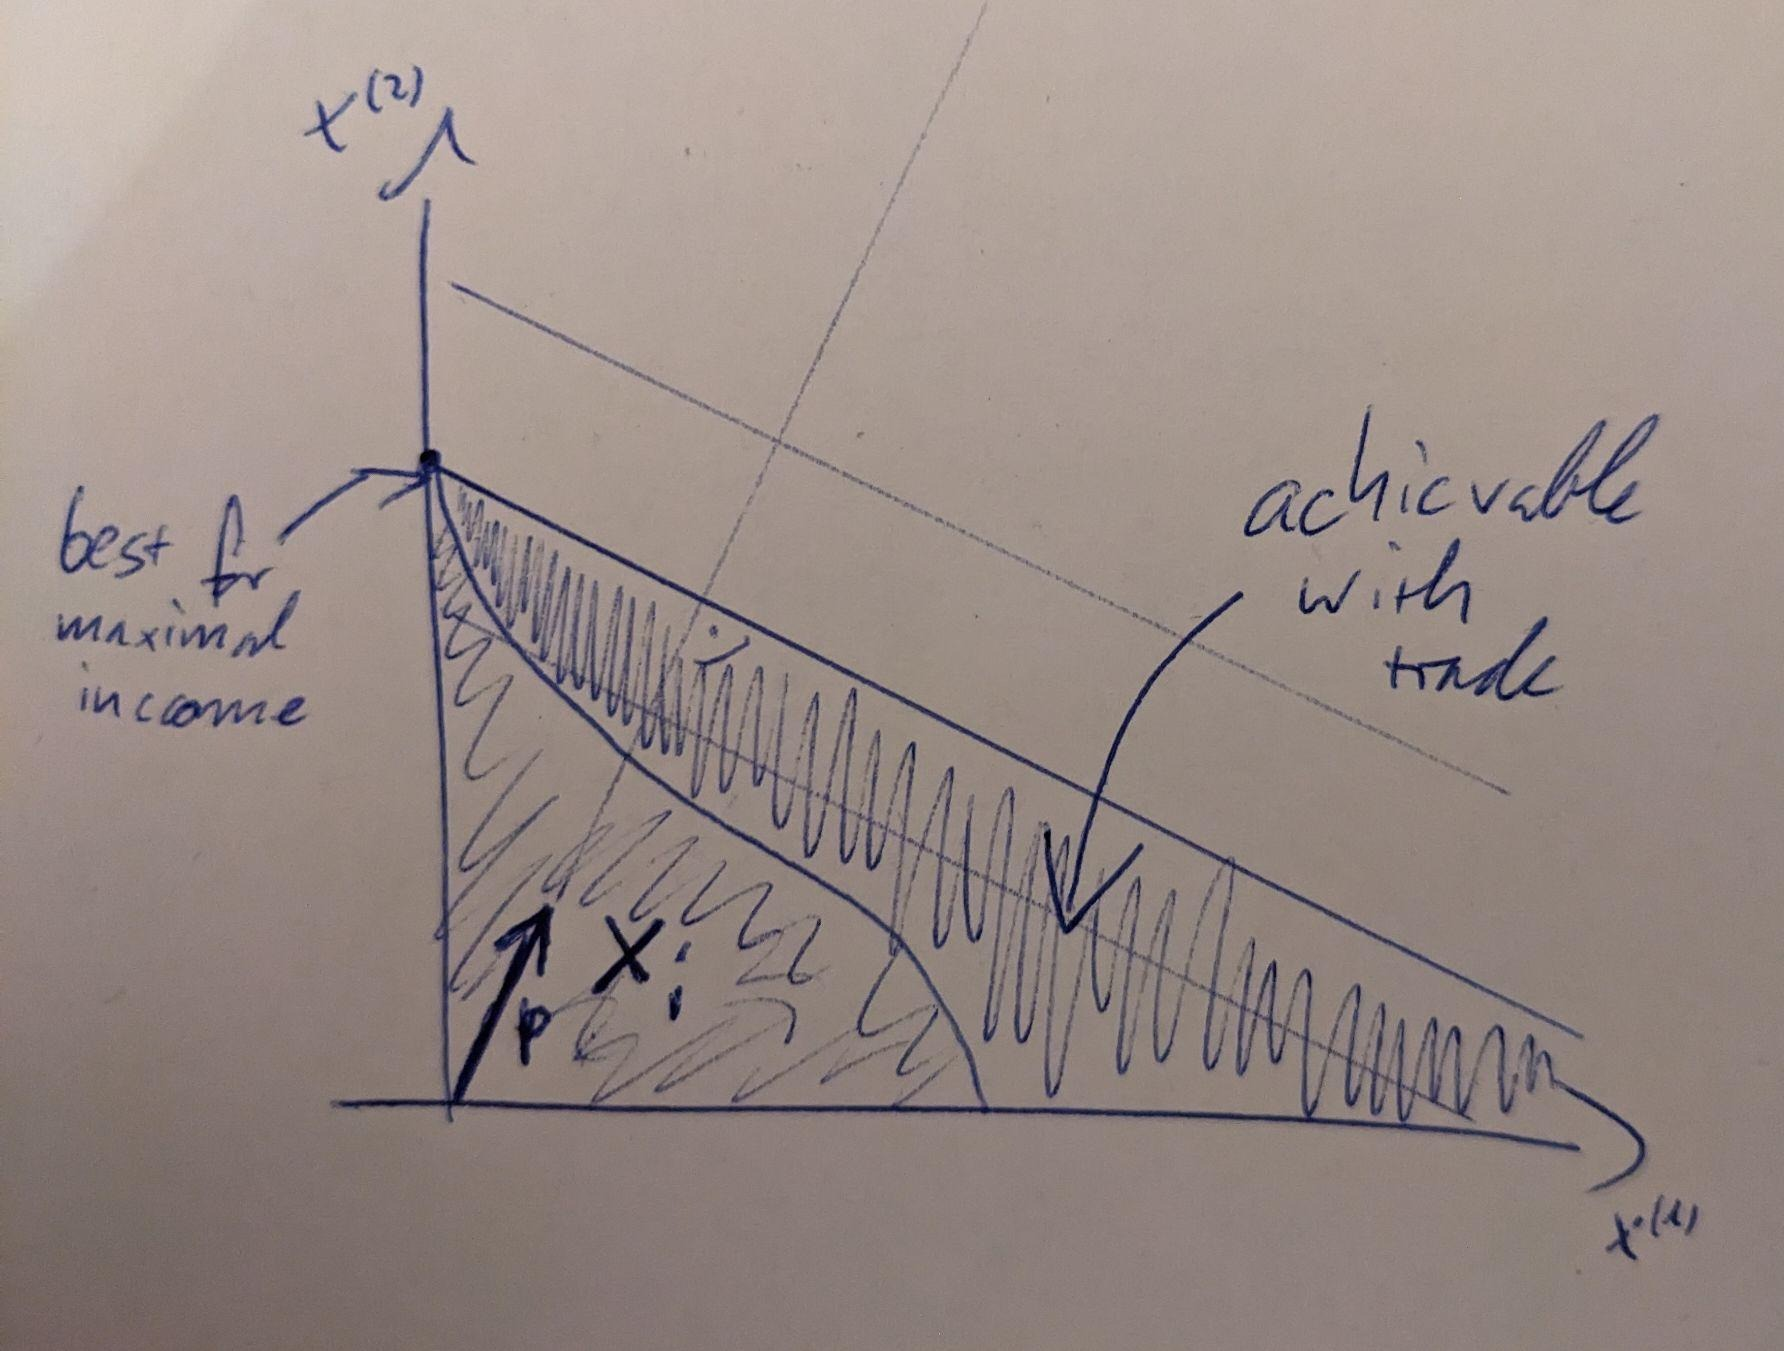
\includegraphics[width=0.7\textwidth]{images/consumption_increase_by_trade.jpeg}
	\caption{
		Product vectors on the \(d-1\) dimensional hyperplanes orthogonal to \(p\)
		cost the same amount and can therefore be exchanged (here \(d=2\), so the
		hyperplanes are lines). Trading at prices \(p\) enlarges the set of
		product vectors available for consumption for person \(i\).
	}
	\label{fig: consumption increase by trade}
\end{figure}
For a fixed price vector \(p\), let us consider the production and consumption
decision of person \(i\). As their expenses have to be smaller than their
income, it makes sense to maximize income for a given amount of labour \(L_i\).
Recall that our production options are \(X_i=X_i(L_i)\). So the maximal income
given labour \(L_i\) is
\[
	\tag{income}\label{eq: income}
	\mu(p, X_i) := \sup\{\langle p, x\rangle : x\in X_i\}.
\]
The function \(\mu(\cdot, X_i)\) in \(p\), is called the ``support function'' of
\(X_i\). It has some useful properties we will be grateful for later on. The
individual decision problem of person \(i\) therefore becomes
\begin{equation}
	\tag{IDP}
	\label{eq: individual decision problem}
	\max_{L_i, y} u(1-L_i, y) \quad\text{s.t.}\quad
	\langle y, p\rangle \le \mu(p, X_i(L_i))
\end{equation}
In Figure~\ref{fig: consumption increase by trade} we can see, how this
constraint is always weaker than \(y\in X_i(L_i)\), which is the constraint of
self-sufficiency. I.e. we get the following lemma.

\begin{lemma}[Trade is never harmful]
\[
	\underbrace{X_i(L_i)}_{\text{own production}}
	\subseteq \quad
	\underbrace{
		\{y\in\real_{\ge 0}^\dims: \langle y, p\rangle \le \mu(p, X_i)\}
	}_{\text{consumption options with trade}}
\]
\end{lemma}
\begin{proof}
	Choose an arbitrary \(y\in X_i\), then by definition of \(\mu\)
	\[
		\langle p, y\rangle \overset{y\in X_i}\le \sup\{\langle p, x\rangle : x\in
		X_i\} \overset{\text{def.}}= \mu(p, X_i),
	\]
	\(y\) is also in the set on the right.
\end{proof}

\subsubsection{Income in the Pure Variable Cost Case}

\begin{lemma}[Income in the Pure Variable Cost Case]
	In the pure variable cost case \(L_i(x) = \langle l_i, x\rangle\), income
	can be written as
	\[
		\mu(p, X_i(L_i))
		= \overbrace{L_i}^{\text{work time}} \max_{j=1,\dots,\dims}
		\underbrace{\frac{p_j}{l_i^{(j)}}}_{=: w_i^{(j)}}
		= L_i \overbrace{\|w_i\|_\infty}^{\text{wage}},
	\]
	where \(w_i^{(j)}\) are potential wages for producing good \(j\).
\end{lemma}
\begin{proof}
	Let \(H:= \diag(l_i)\), then as \(X_i\) is compact we know the supremum is
	a maximum and
	\begin{align*}
		\mu(p, X_i)
		&= \max_{x\ge 0} \langle p, x\rangle
		\text{ s.t. } \langle x, l_i\rangle \le L_i\\
		&\overset{y=Hx}= \max_{y\ge 0} \langle p, H^{-1}y\rangle
		\text{ s.t. } \underbrace{\langle H^{-1}y, l_i\rangle}_{
			= \langle y, 1 \rangle = \|y\|_1
		} \le L_i\\
		&= L_i \underbrace{
			\max_{y\ge 0} \langle H^{-1}p, y\rangle \text{ s.t. } \|y\|_1 \le 1
		}_{
			= \|H^{-1} p\|_{\text{Op-Norm(1)}} = \|H^{-1} p \|_\infty
		}\\
		&= L_i \max_{j=1,\dots,\dims} \frac{p_j}{l_i^{(j)}},
	\end{align*}
	where we have used, that all entries of \(y\) are non-negative when
	converting to the \(1\)-norm, \(\|x\|_1 = \sum_{i=1}^\dims |x_i|\), the
	fact that the operator norm of the \(1\)-norm is the sup norm
	\(\|x\|_\infty = \sup_{i=1,\dots,\dims} |x_i|\)\fxnote{source or appendix},
	and finally positivity of entries of \(p\) and \(l_i\) again.
\end{proof}

\subsubsection{Income with Fixed Costs}

While the pure variable cost case already lends itself to specialization, unless
multiple wage options \(w_i^{(j)}\) are identical, adding fixed costs truly
encourages specialization. For fixed costs \(f_i\) the production capability
of person \(i\) can be written as 
\[
	X_i = \{
		x\in \real_{\ge 0}^\dims
		: \langle l_i, x\rangle
		+ \underbrace{
			\sum_{j=1}^\dims f_i^{(j)}\ind_{x^{(j)}>0}
		}_{=: \langle f_i, \ind_{>0}\rangle} \le L_i
	\}.
\]

\begin{lemma}[Income in Variable \& Fixed Cost Case]
	We assume the person is able to produce any product. So none of the fixed
	costs \(f_i^{(j)}\) take longer than the total labour time \(L_i\) (i.e.
	\(L_i - f_i^{(j)} > 0\)). In this mixed case, income of person \(i\) can be
	written as		
	\[
		\mu(p, X_i)
		= L_i \max_{j=1,\dots,d}
		\underbrace{\frac{p_j}{\bar{l}_i^{(j)}}}_{=:w_i^{(j)}}
		= L_i \|w_i\|_\infty,
	\]
	where the average labour cost \(\bar{l}_i^{(j)}\) of person \(i\) of
	specialization \(j\) is given by
	\[
		\bar{l}_i^{(j)}
		:= l_i^{(j)}\frac{L_i}{L_i-f_i^{(j)}}
		= l_i^{(j)}\frac{1}{1-f_i^{(j)}/L_i}
	\]
\end{lemma}
\begin{proof}
	For a subset \(J\subseteq\{1,\dots,\dims\}\) define the subspace
	\[
		\real_{>0}^J:= \{
			x\in \real^\dims:
			x^{(j)} > 0\ \forall j\in J;\;\; x_j =0\ \forall j\notin J
		\}.
	\]
	Then we can partition our maximization problem by these \(J\) like this:
	\begin{align*}
		\mu(p, X_i)
		&= \max_{x\ge 0}\langle p, x\rangle \text{ s.t. }
		\langle x, l_i\rangle  + \langle f_i, \ind_{>0}\rangle \le L_i\\
		&= \max_{J \subseteq \{1,\dots,\dims\}}
		\max_{x\in \real_{>0}^J}
		\langle p, x\rangle \text{ s.t. }
		\langle x, l_i\rangle \le L_i - \sum_{j\in J}f_i^{(j)}
	\end{align*}	
	We can relax the inner maximization problem to obtain the pure variable
	optimization problem embedded in \(\real^I\)
	\begin{align*}
		&\max_{x\in \real_{>0}^J}
		\langle p, x\rangle \text{ s.t. }
		\langle x, l_i\rangle \le L_i - \sum_{j\in J}f_i^{(j)}\\
		&\le 
		\max_{x\in \real_{{\color{red} \ge} 0}^J}
		\langle p, x\rangle \text{ s.t. }
		\langle x, l_i\rangle \le L_i - \sum_{j\in J}f_i^{(j)}\\
		&= \Bigl(L_i - \sum_{j\in J}f_i^{(j)}\Bigr)
		\max_{j\in J} \frac{p_j}{l_i^{(j)}}
	\end{align*}
	So in total, we have
	\begin{align*}
		\mu(p, X_i)
		&\le \max_{\emptyset \neq J\subseteq \{1,\dots,\dims\}}
		\Bigl(L_i - \sum_{j\in J}f_i^{(j)}\Bigr)
		\max_{j\in J} \frac{p_j}{l_i^{(j)}}\\
		&= \max_{j=1,\dots,\dims}
		(L_i - f_i^{(j)}) \frac{p_j}{l_i^{(j)}}.
	\end{align*}
	To see that this upper bound is actually tight, consider producing
	exclusively \(j\). Then we have
	\[
		l_i^{(j)} x^{(j)} + f_i^{(j)} = L_i \iff x^{(j)}
		= \frac{L_i-f_i^{(j)}}{l_i^{(j)}}.
	\]
	Optimizing over different specializations yields
	\[
		\mu(p, X_i) \ge \max_{j=1,\dots,\dims} p_j x^{(j)}
		= \max_{j=1,\dots,\dims}
		p_j \frac{L_i - f_i^{(j)}}{l_i^{(j)}}
		= L_i\max_{j=1,\dots,\dims}
		\frac{p_j}{l_i^{(j)}\frac{L_i}{L_i - f_i^{(j)}}}.
	\]
	Lastly the average labour cost of specialization \(j\) is given by
	\begin{align*}
		\bar{l}_i^{(j)}
		&= \frac{L_i}{x^{(j)}}
		= \frac{l_i^{(j)} x^{(j)} + f_i^{(j)}}{x^{(j)}}
		= l_i^{(j)} + \frac{f_i^{j}}{\left(\frac{L_i-f_i^{(j)}}{l_i^{(j)}}\right)}
		= l_i^{(j)} \Bigl[1 + \frac{f_i^{j}}{L_i-f_i^{(j)}}\Bigr]\\
		&=l_i^{(j)}\frac{L_i}{L_i - f_i^{(j)}}.
		\qedhere
	\end{align*}
\end{proof}

\subsubsection{The Individual Decision Problem in the Mixed Case}

By talking about average costs \(\bar{l}_i^{(j)}\) in place of variable costs
\(l_i^{(j)}\), we salvaged the results from the pure variable
cost case. But no matter how the wage \(\|w_i\|_\infty\) comes to be, the
individual decision problem \eqref{eq: individual decision problem} becomes
\[
	\max_{L_i, y} u(1-L_i, y) \text{ s.t. } \langle p, y\rangle \le L_i \|w_i\|_\infty
\]
or in other words
\[
	\max_{y} u\left(1- \frac{\langle p, y\rangle}{\|w_i\|_\infty}, y\right).
\]
The first order condition is therefore
\[
	\frac{du}{dy} 
	= u_f\Bigl[
		\underbrace{\frac{u_y}{u_f}}_{\text{wtw}}
		- \overbrace{\frac{p}{\|w_i\|_\infty}}^{\text{effort required}}
	\Bigr]
	= \frac{u_f}{\|w_i\|_\infty}\Bigl[
		\underbrace{\frac{u_y}{u_f}\|w_i\|_\infty}_{\text{wtp}}
		- p
	\Bigr]
\]
Where the ``willingness to pay'' (wtp) is simply the willingness to work
(wtw) scaled by person \(i\)'s wages.

Careful readers might have noticed, that
this calculation is not quite accurate in the mixed case. Because the average
costs depend on \(L_i\), which in turn makes \(\|w_i\|_\infty\) dependent on
\(L_i\). So by the product rule, the effort required would be
\[
		\frac{dL_i}{dy}
		= \frac{d}{dy} \frac{\langle p, y\rangle}{\|w_i\|_\infty}
		= \frac{p}{\|w_i\|_\infty}
		- \frac{\langle p, y\rangle}{\|w_i\|_\infty^2}
		\frac{d\|w_i\|_\infty}{dL_i}\frac{dL_i}{dy}
\]
Joining the \(\frac{dL_i}{dy}\) on both sides results in
\[
	\frac{dL_i}{dy}
	= \frac{\frac{p}{\|w_i\|_\infty}}{
		1 + \frac{\langle p, y\rangle}{\|w_i\|_\infty^2}
		\frac{d\|w_i\|_\infty}{dL_i}
	}
	= \frac{p}{
		\|w_i\|_\infty + \frac{\langle p, y\rangle}{\|w_i\|_\infty}
		\frac{d\|w_i\|_\infty}{dL_i}
	}.
\]
Where \(\|w_i\|_\infty=\max_{j} w_i^{(j)}\) is piecewise differentiable with
derivatives
\[
	\frac{dw_i^{(j)}}{dL_i}
	= \frac{d}{dL_i} \frac{p_j}{\bar{l}_i^{(j)}}
	= \frac{p_j}{l_i^{(j)}} \frac{d}{dL_i} \frac{L_i-f_i^{(j)}}{L_i}
	= \frac{p_j}{l_i^{(j)}} \frac{f_i^{(j)}}{L_i^2} > 0.
\]
In other words: Wages increase with total labour time \(L_i\), as
average cost decrease with \(L_i\). The size of this effect increases with the
size of the fixed costs. If the fixed costs are close to \(L_i\) small decreases
of \(L_i\) might make producing \(j\) completely unviable, but at the very least
cut heavily into the little time left for actually producing \(j\). In fact
average costs have singularities at \(f_i^{(j)}\)
\[
	\lim_{L_i\downarrow f_i^{(j)}} \bar{l}_i^{(j)}
	= \lim_{L_i\downarrow f_i^{(j)}}l_i^{(j)}\frac{1}{1-f_i^{(j)}/L_i}
	= \infty.
\]
Using \(\bar{l}_i^{(j)}=l_i^{(j)}\frac{L_i}{L_i-f_i^{(j)}}\) we can alternatively
write
\[
	\frac{dw_i^{(j)}}{dL_i}
	= \frac{p_j}{\bar{l}_i^{(j)}} \frac{f_i^{(j)}(L_i-f_i^{(j)})}{L_i}
	= w_i^{(j)} \frac{f_i^{(j)}(L_i-f_i^{(j)})}{L_i}.
\]
With \(j^* := \argmax_{j} w_i^{(j)}\) and \(L_i = \frac{\langle p,
y\rangle}{\|w_i\|_\infty}\), this finally results in the effort required
\[
	\frac{dL_i}{dy}
	= \frac{p}{
		\|w_i\|_\infty + \langle p, y\rangle f_i^{(j^*)}
		\bigl(1-\frac{f_i^{(j^*)}}{L_i}\bigr)
	}
	= \frac{p}{
		\|w_i\|_\infty + f_i^{(j^*)}
		\bigl(\langle p, y\rangle-f_i^{(j^*)}\|w_i\|_\infty\bigr)
	}.
\]
The willingness to pay is therefore given by
\[
	\text{wtp} = \frac{u_y}{u_f}\Bigl[
		\|w_i\|_\infty + f_i^{(j^*)}
		\bigl(\langle p, y\rangle-f_i^{(j^*)}\|w_i\|_\infty\bigr)
	\Bigr].
\]

\subsection{Prices in Societies of Clones}

Let us consider the mixed cost case and assume that everyone has the exact same
production capabilities (i.e. \(\bar{l}^{(j)} = \bar{l}_i^{(j)}\) for all
\(i\)). Then everyone's potential wages are identical
\[
	w_i^{(j)} = \frac{p_j}{\bar{l}^{(j)}} =: w^{(j)}.
\]
People will therefore only produce good \(j\) if \(w^{(j)} = \| w\|_\infty\).
If a society wants to consume a little of every good, every good needs to be
produced. But this implies all \(w^{(j)}\) have to be identical to
\(\|w\|_\infty\). This implies
\[
	\|w\|_\infty = \frac{p_j}{\bar{l}^{(j)}},
\]
and thus \(p_j = \bar{l}^{(j)}\|w\|_\infty\). Up to the factor \(\|w\|_\infty\)
of wages, we therefore fully determined prices. And as we argued in
Section~\ref{subsec: money supply and price stability}, we lose this degree of
freedom to the money supply. In fact by
\[
	\langle p, S\rangle = MV = \text{GDP}
\]
we can determine wages to be
\[
	\|w\|_\infty = \frac{\text{GDP}}{\langle \bar{l}, S\rangle}
	= \frac{\text{sum of money transactions}}{\text{time required to produce }S}.
\]
Where the transactions might be denoted in \$, the time might be denoted in
hours \(h\) and the wage is therefore denoted in \(\$/h\). Notice how
\(60 \text{min}/h\) has almost the same format. This is no coincidence. Since
everyone takes the same amount of time \(\bar{l}^{(j)}\) to produce good \(j\)
the \(\$\) value is literally a unit of time.

Once you break the assumption that all \(\bar{l}_i^{(j)}\) are identical, this
ceases to be the case. An easy generalization is when \(\bar{l}_i^{(j)}\) are
simply multiples of one another. In this case, the wage options are also
multiples. So we still need to require that they are all equal otherwise some 
good is not produced. This finally results in
\[
	p_j = \bar{l}_i^{(j)}\|w_i\|_\infty.
\]
In this case \(\|w_i\|_\infty\) can still be used as a subjective unit of time
(different for every person \(i\)).

The takeaway is: if it is obvious how the effort behind good \(j\) should be
valued, then the only price equilibrium is in fact this obvious valuation.
Prices should therefore be viewed as measures of effort.

But typically people are not just better in everything. Which means that the
measure of value \(p\) will finally need to depart from the measure of time
\(\bar{l}_i\).

\subsection{Intuition in 2D for the Mixed Case}

\FloatBarrier
Before we move to abstract general equilibrium theory, let us build some
intuition with pictures.

\begin{figure}
	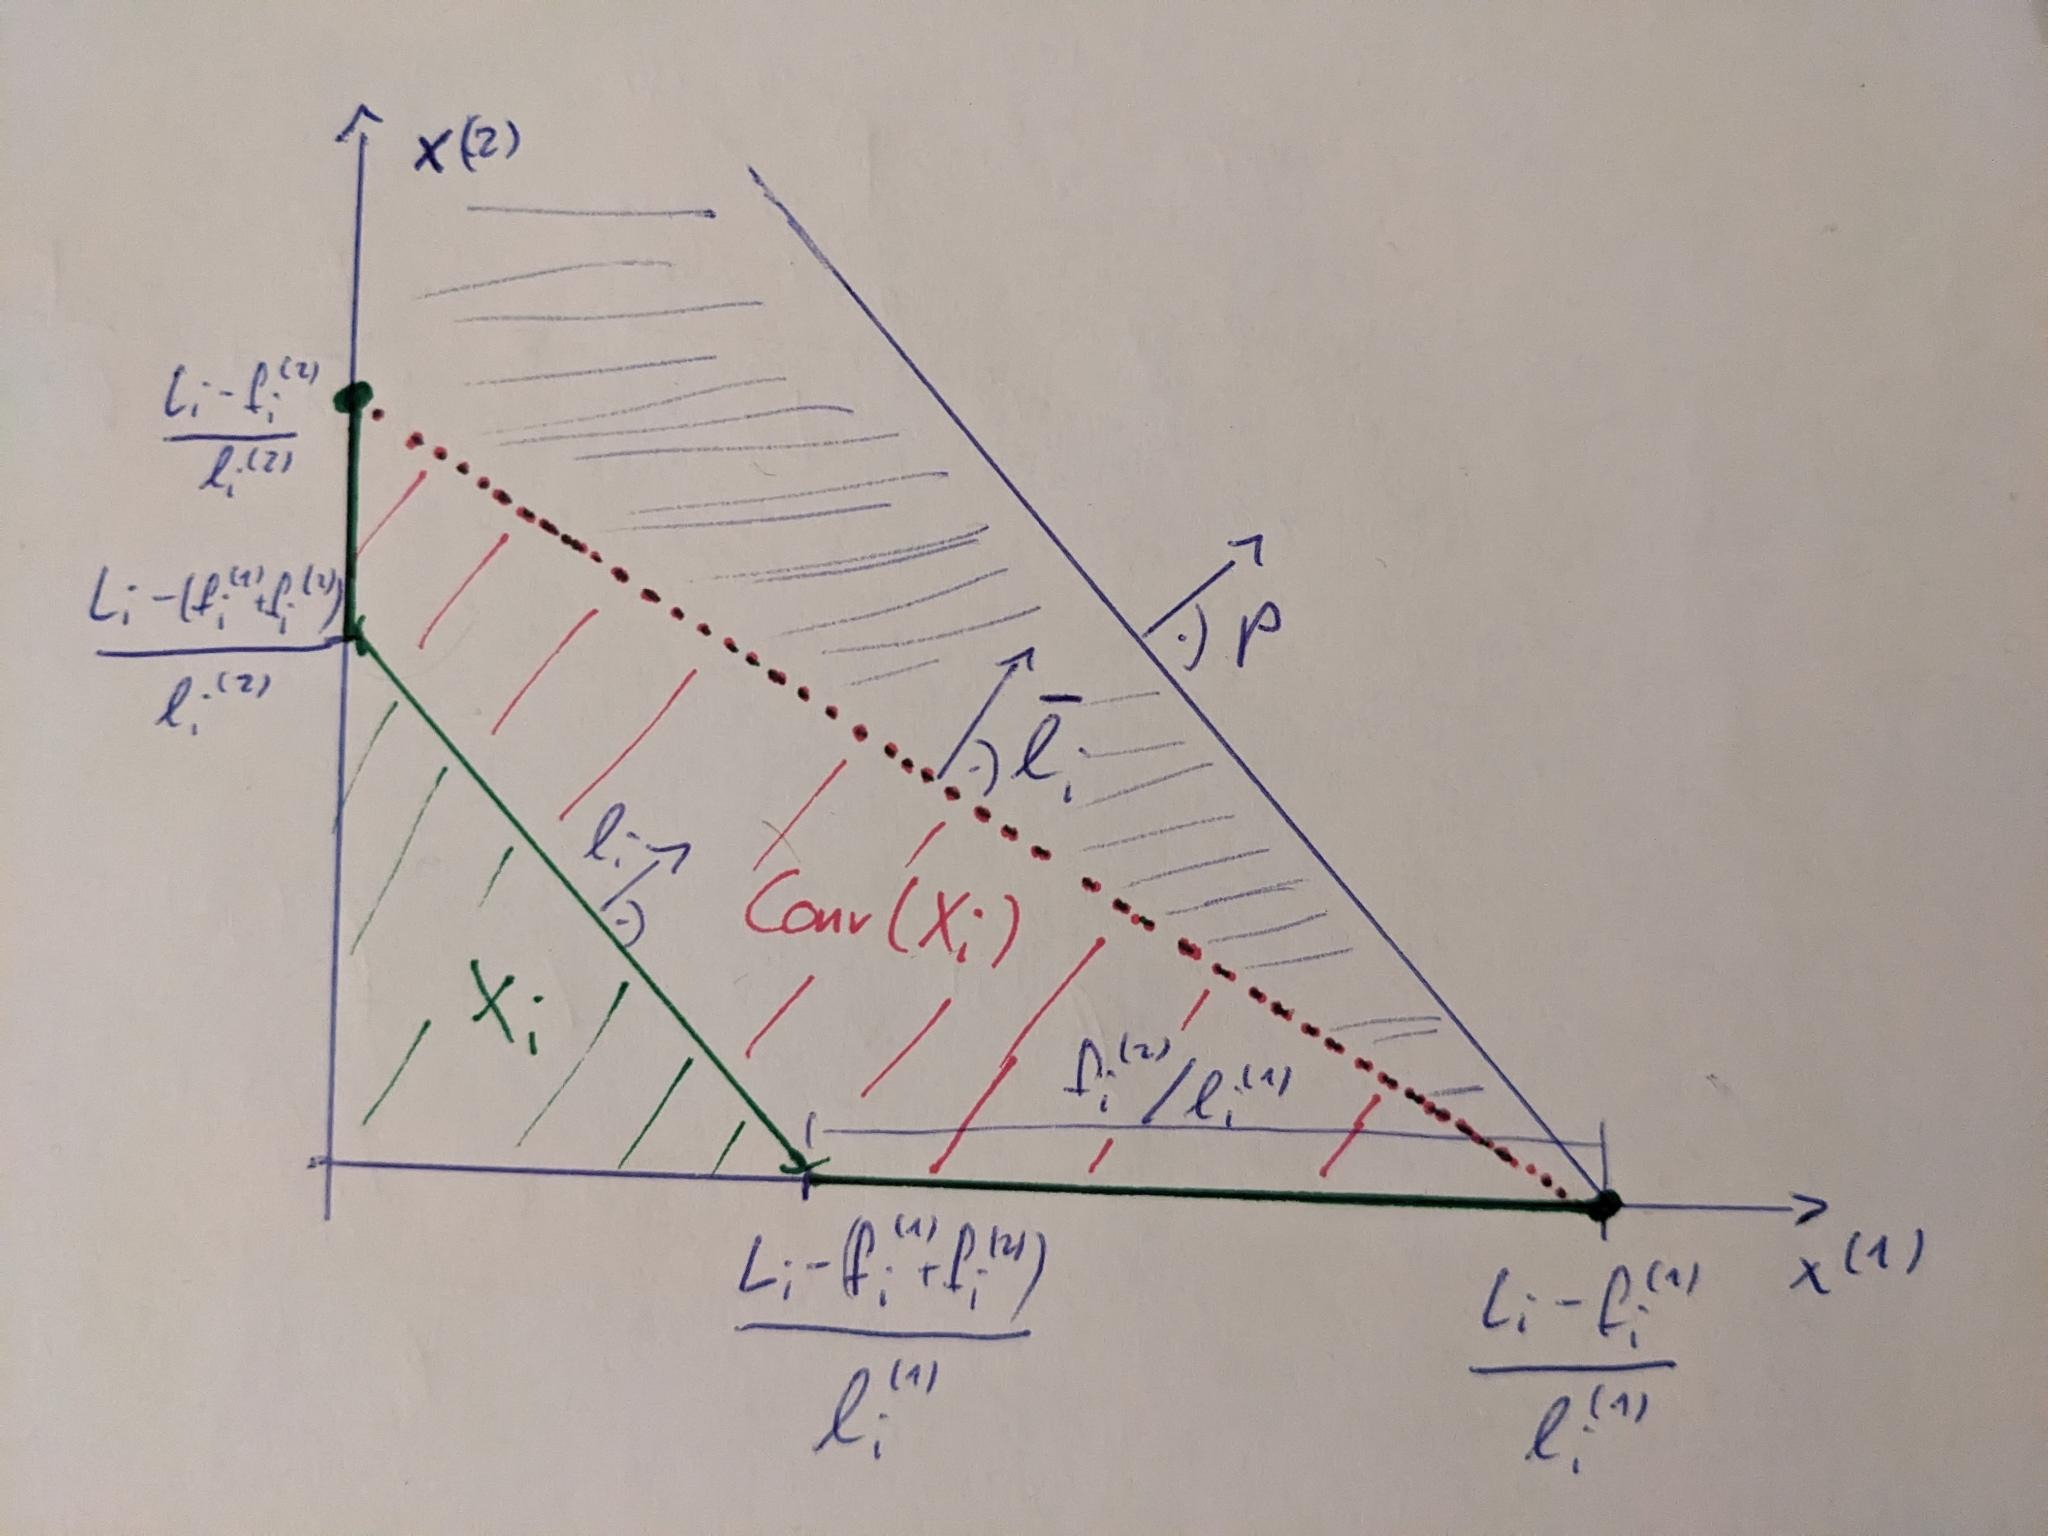
\includegraphics[width=0.95\textwidth]{images/conv_hull_vs_trade.jpeg}
	\centering
	\caption{
		The convex hull \(\conv(X_i)\) is larger than \(X_i\). But trade might
		be an improvement even still. Trade is always at least as good as the
		convex hull. The more different \(p\) from \(\bar{l}_i\) the better for
		individual \(i\). If \(p\) and \(\bar{l}_i\) were equal only
		\(\conv(X_i)\) would be available for consumption.
	}
\end{figure}

\begin{figure}
	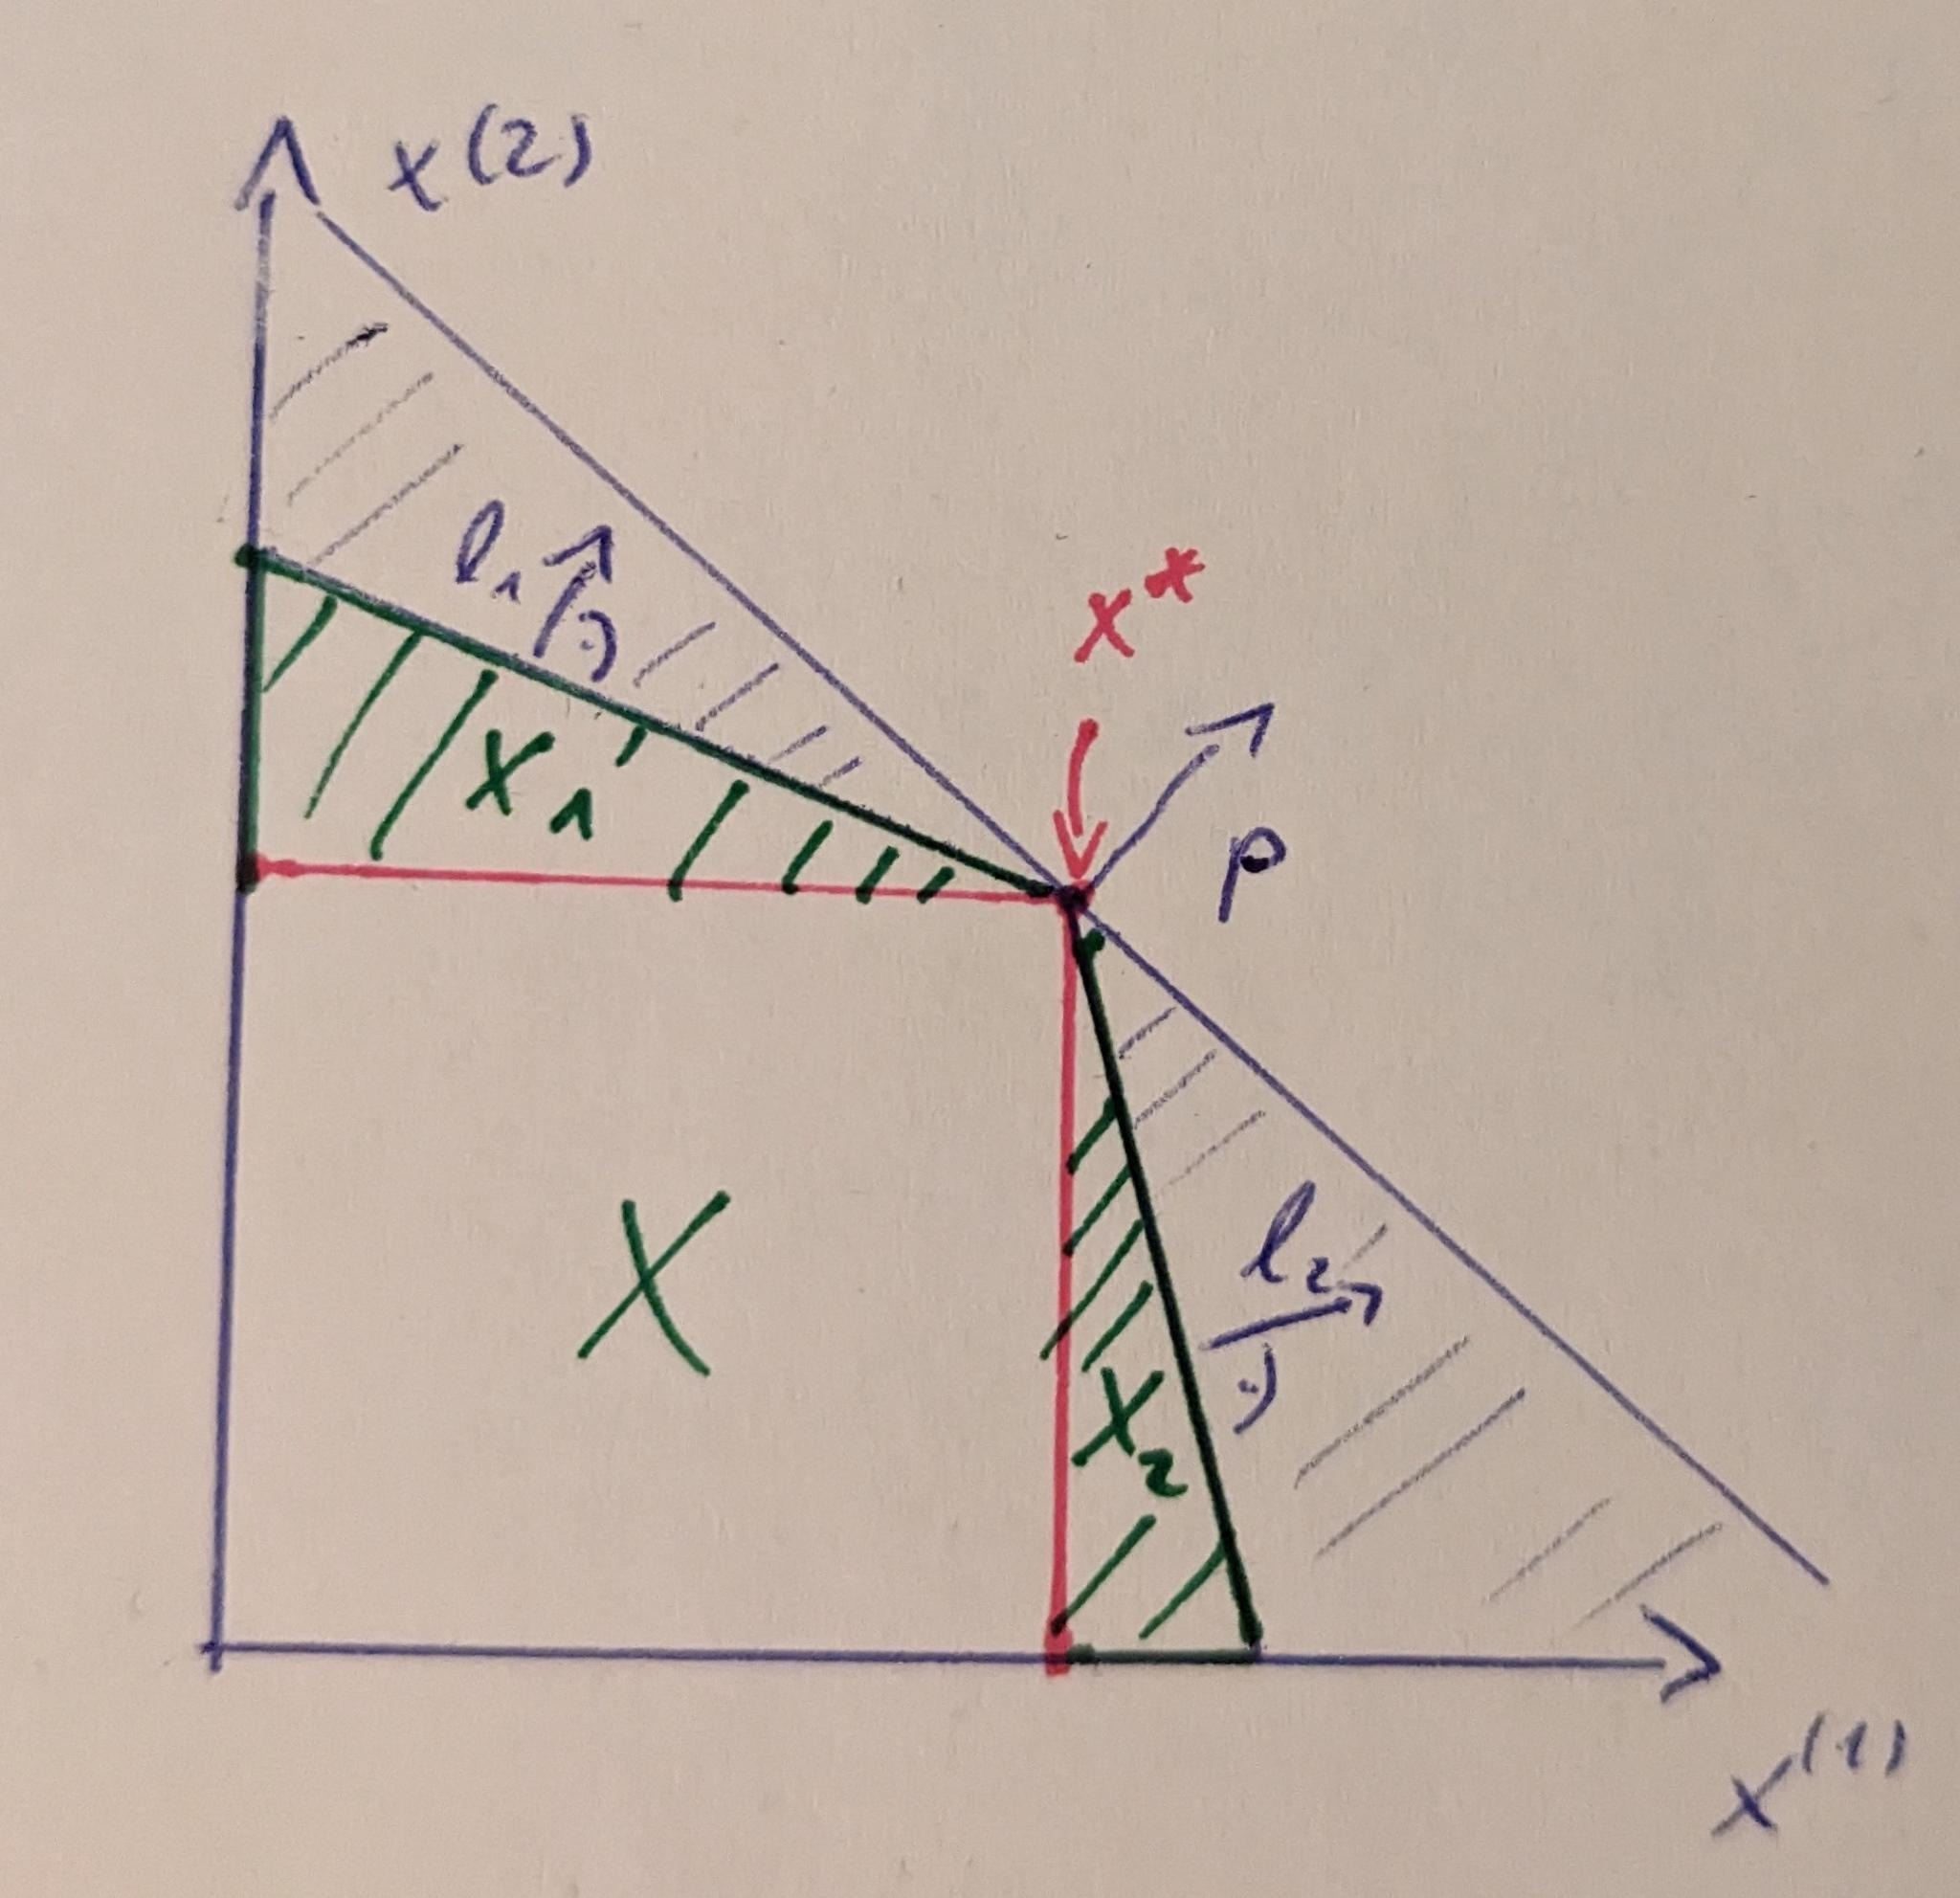
\includegraphics[width=0.3\textwidth]{images/2_people_trade_fair.jpeg}
	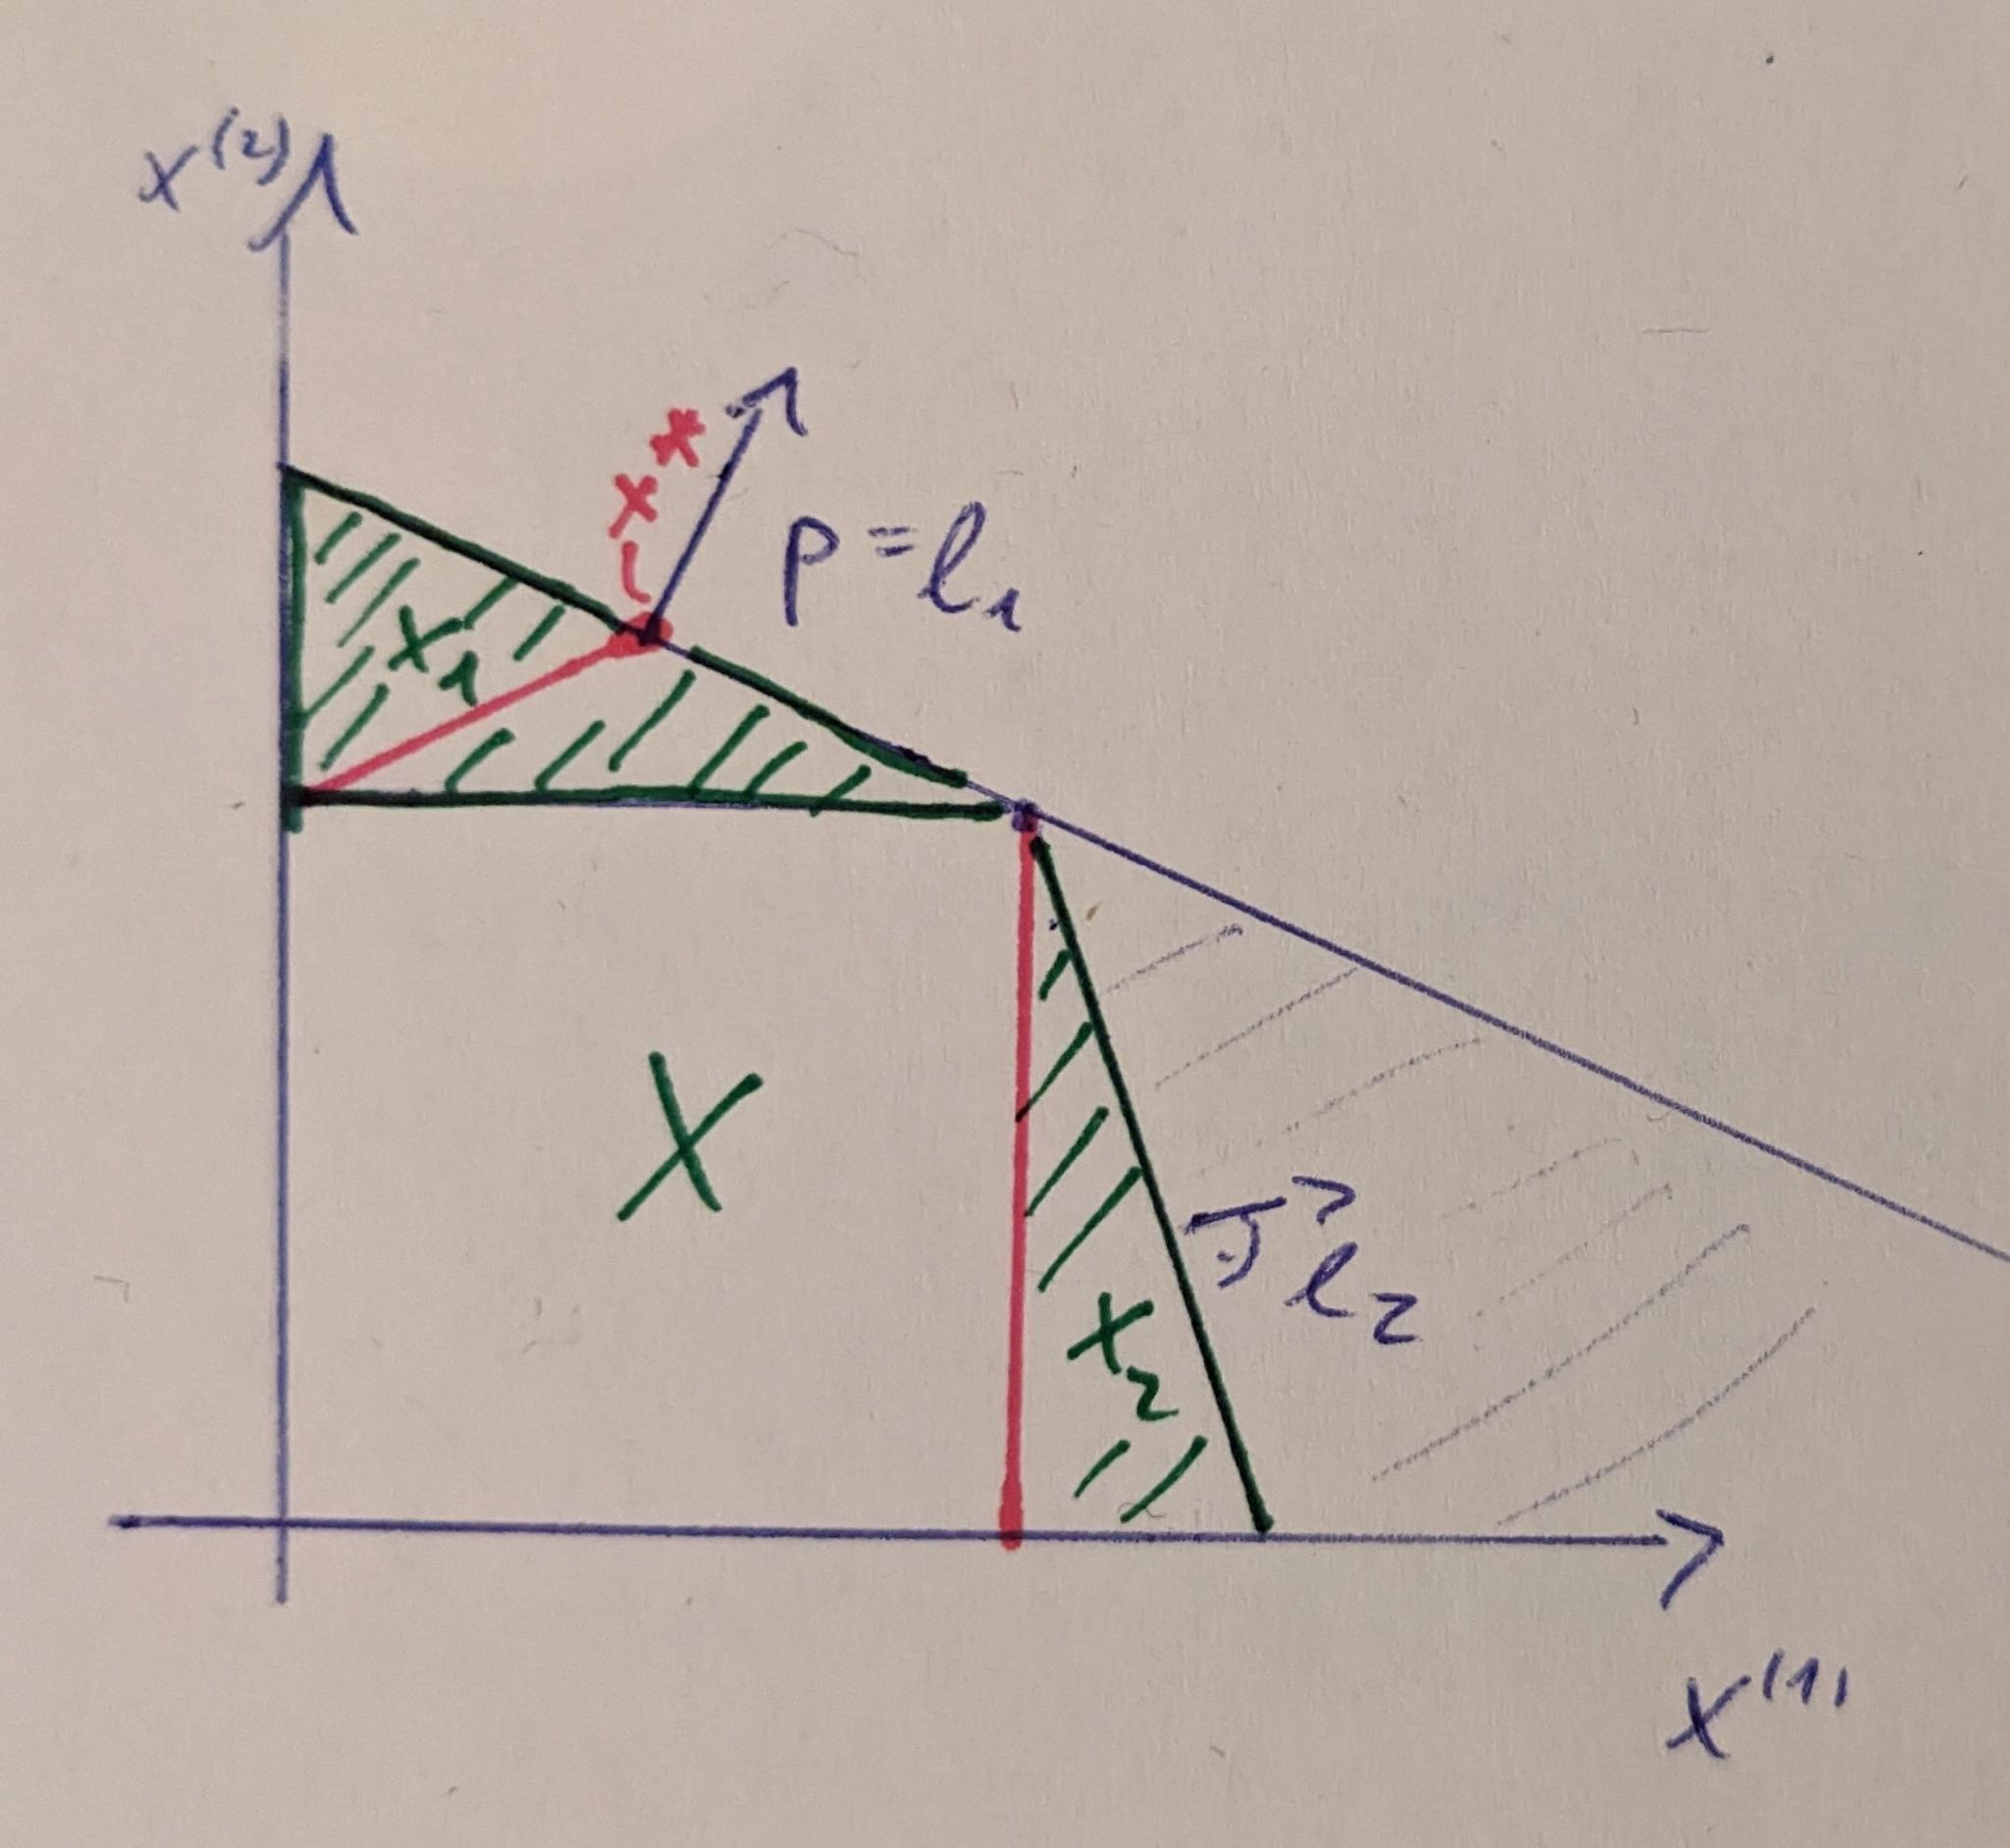
\includegraphics[width=0.315\textwidth]{images/2_people_trade_half_specialization.jpeg}
	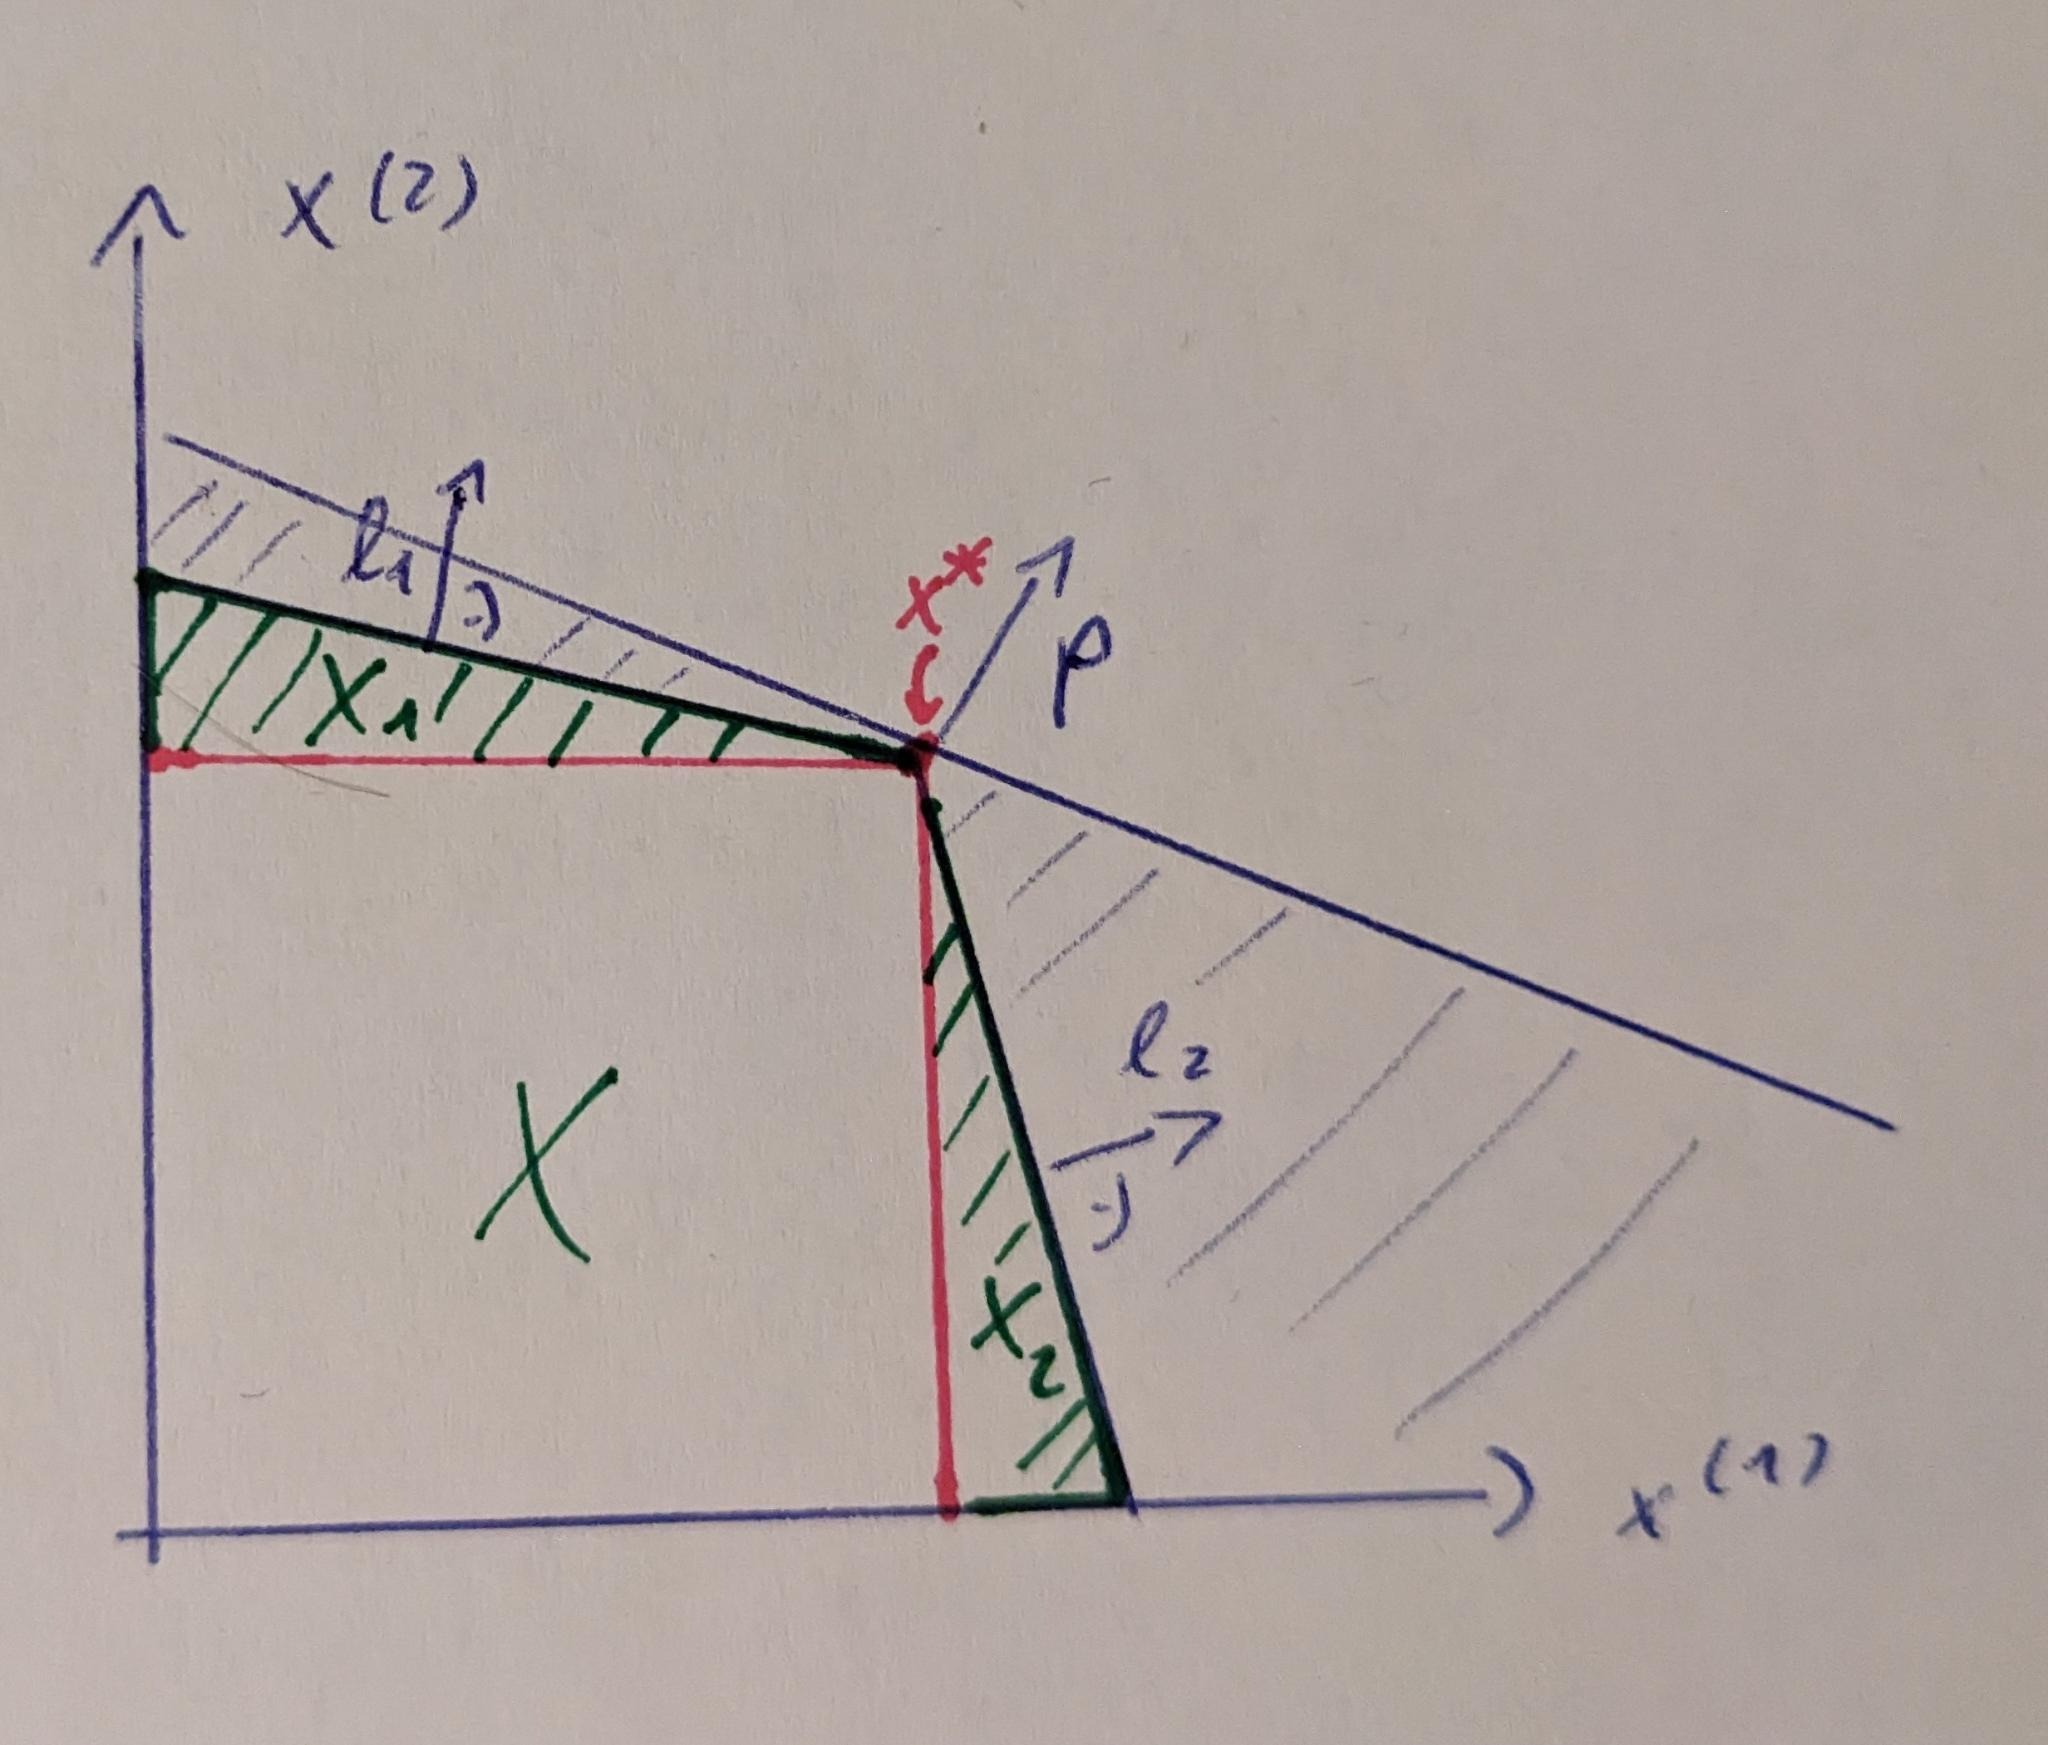
\includegraphics[width=0.34\textwidth]{images/2_people_trade_unfair.jpeg}
	\caption{
		Two people with different skills producing \(x^*\) together. In the first
		picture person \(i\) specializes on producing \(i\) and they both gain
		from this trade as \(p\) is different from \(l_i\). In the second picture,
		person \(1\) produces both goods. The price vector has to be a multiple of
		\(l_1\), otherwise person \(1\) would focus on one of the two goods.
		Person \(1\) does not gain anything from trade. In the third picture, both
		are specialized and both gain from trade, but the gains of person \(2\)
		are larger than person \(1\) as \(p\) is closer to \(l_1\) in direction.
	}
\end{figure}

\begin{figure}
	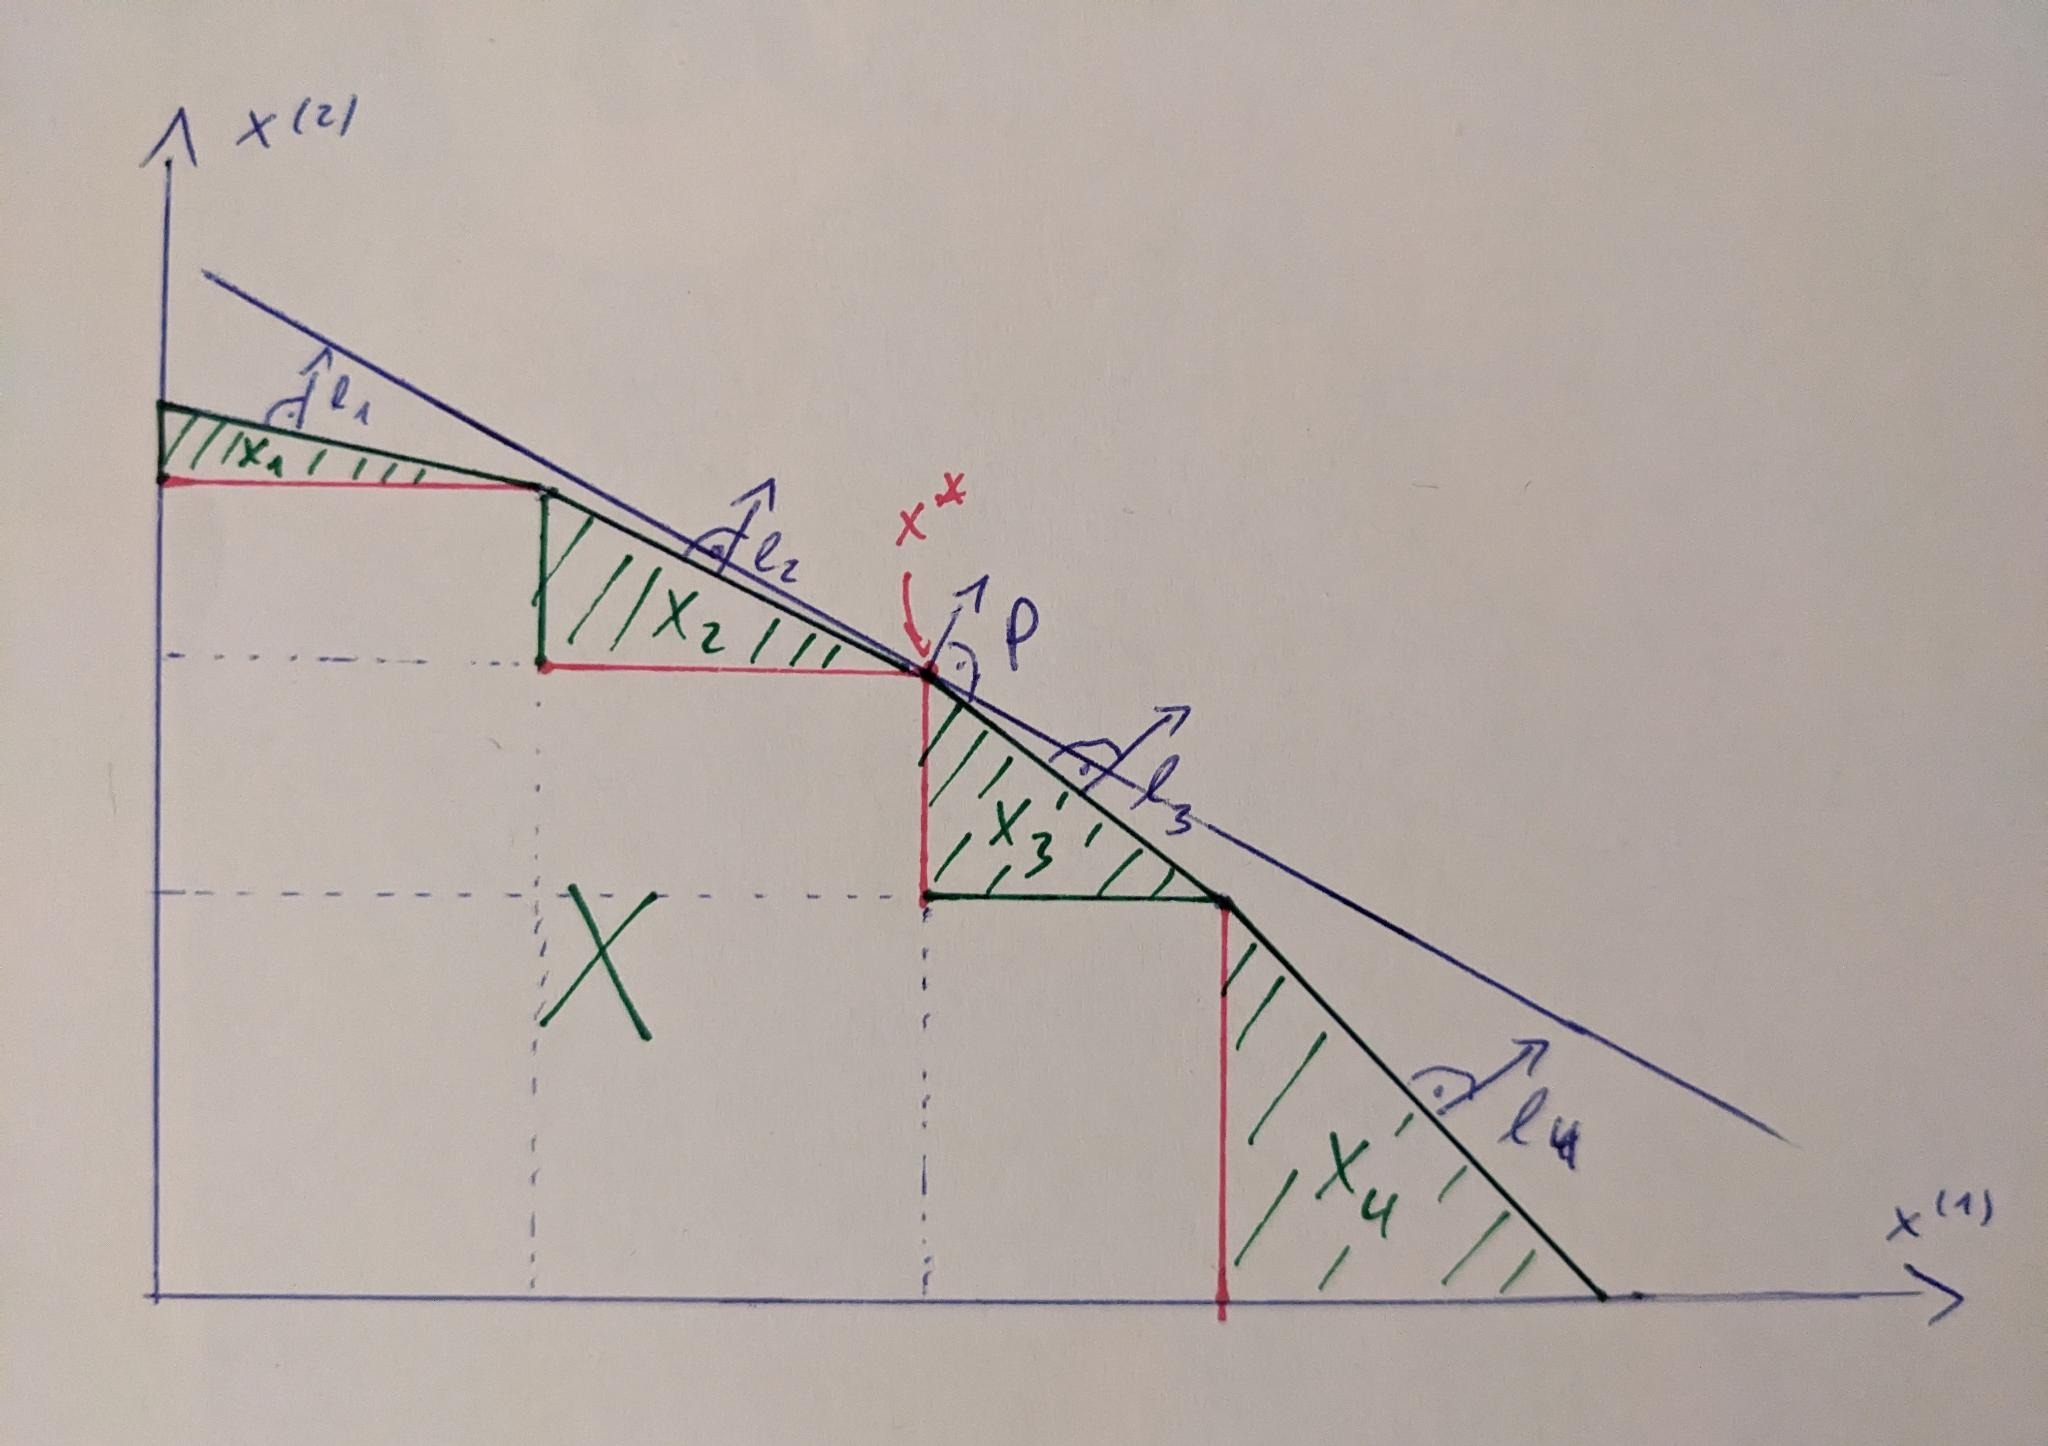
\includegraphics[width=0.95\textwidth]{images/4_people_trade.jpeg}
	\caption{
		Four people are producing \(x^*\) together. The more specialized people
		on the edges \(1,4\) gain more from this trade than the people in the
		middle, where \(p\) is more similar to \(l_i\). The more people you add
		the, smoother the border of \(\bar{X}_n\) should become. The edges
		give us the opportunity to pick \(p\) in a range of the adjacent \(l_i\).
		A smooth border would give us no choice, as \(p\) would have to be
		tangential. Also notice that fixed costs for individuals matter less and
		less with more people, as almost nobody needs to produce more than one
		good. For this essentially remove the upper right part of the triangles
		of the \(X_i\) and observe that the points on the outer surface would
		still move together and become a continuous curve for large numbers of
		people.
	}	
\end{figure}

You should get the intuition that we can achieve any \(x^*\) in the ``production
frontier'' of \(X\) (we will define properly later) with positive prices from
these pictures. And that this price is essentially fully determined if enough
people participate (which will be the topic of Section~\ref{sec: demand & supply
dist functions}). Lastly you should understand how people would like prices to
be dissimilar to their own skills. Highly specialized people gain more from
trade than generalists.

\FloatBarrier
	\section{Production Frontier}

We define the production frontier as the set of points which can not be
achieved by producing a different vector and then throwing away things:
\[
	\pf(X) := \{ x\in X : \nexists y\in X \text{ with } x\prec y\}
\]
where \(x\prec y\) is defined to be \(x^{(i)} \le y^{(i)}\) for all \(i\) and
there exists at least one \(i\) where the inequality is strict.

\begin{lemma}[Production Frontier is part of the Boundary of X]
	\label{lem: prod frontier part of boundary}
	\[
		\pf(X)\subseteq \partial X
	\]
\end{lemma}
\begin{proof}
	For any \(x=(x^{(1)},\dots, x^{(\dims)})\in X^\circ\) exists \(\epsilon>0\)
	such that \(x_{+\epsilon} = (x^{(1)}+\epsilon, \dots, x^{(\dims)}+\epsilon)\)
	is an element of \(X\). But then \(x\) can not be an element of \(\pf(X)\),
	since \(x \prec x_{+\epsilon}\).
\end{proof}

To characterize the production frontier further, we are going to assume
convexity of \(X\). We have motivated the asymptotic convexity of the
average production capabilities \(\bar{X}_n\) in Lemma~\ref{lem: clone prod
cap}. While this asymptotic convexity does not translate to convexity of \(X\)
one could easily replace \(X\) with \(\bar{X}_n\) in the following, at the
expense of notational simplicity.

\begin{lemma}[Duality of Support Function]
	\label{lem: duality of support function}
	If \(X\) is a compact, convex \ref{eq: lower
	layer}, then for any \(x\in \partial X\), there exists
	\(p\neq 0\) such that
	\begin{equation}
		\label{eq: prod frontier p}
		x \in \argmax_{y\in X} \langle p, y\rangle %= \nabla_p \mu(p, X)
	\end{equation}
	and therefore
	\[
		\mu(p, X) = \langle p, x\rangle.
	\]
	If additionally \(x\in\real_{>0}^\dims\), then necessarily \(p\in\real_{\ge
	0}^\dims\) if \(p\) satisfies \eqref{eq: prod frontier p}.
\end{lemma}
\begin{proof}
	Let \(x\in \partial X\), define \(A:=X^\circ\) and \(B:=\{x\}\). Then \(A\)
	is open; \(A\) and \(B\) are disjoint, nonempty
	convex subsets of \(\real^\dims\). So by the hyperplane separation theorem
	there exists
	\(0\neq p\in\real^\dims\) and \(c\in\real\) with
	\[
		\forall y\in A : \langle y, p\rangle < c
		\qquad\text{and}\qquad
		\langle x, p\rangle \ge c.
	\]
	Due to continuity of the scalar product we also have \(\langle y, p\rangle
	\le c\) for all \(y\in X\). Since \(x\in X\) this implies
	\begin{equation}
		\label{eq: x is max w.r.t. p}
		\langle y, p\rangle \le c = \langle x, p\rangle \quad \forall y\in X
	\end{equation}
	Therefore \(x\in\argmax_{y\in X} \langle p, y\rangle\) and \(\mu(p, X) =
	\langle x, p\rangle\).

	Let us now consider \(x=(x^{(1)},\dots,x^{(\dims)})\in\real_{>0}^\dims\).
	To arrive at a contradiction, we assume \(p_i < 0\). Since \(x^{(i)}>0\) and
	\(X\) is a \ref{eq: lower layer}, we can replace the entry \(x^{(i)}\) with
	\(0\) to obtain \(\tilde{x}\in X\). Then
	\[
		\langle \tilde{x}, p\rangle
		= \sum_{\substack{j=1\\i\neq j}} x^{(j)} p_j
		> \underbrace{x^{(i)}}_{>0}\underbrace{p_i}_{<0}
		+ \sum_{\substack{j=1\\i\neq j}} x^{(j)} p_j
		= \langle x, p\rangle,
	\]
	which is a contradiction to \eqref{eq: x is max w.r.t. p}.
\end{proof}

\begin{theorem}[Production Frontier Characterization]
	If \(X\) is a compact, convex \ref{eq: lower layer}, then
	\[
		\bigcup_{p\in \real_{>0}^\dims} \argmax_{y\in X}\langle p, y\rangle
		\subseteq \pf(X) \subseteq
		\bigcup_{p\in \real_{\ge 0}^\dims\setminus\{0\}}
		\argmax_{y\in X}\langle p, y\rangle.
	\]
	Where the first subset property does not actually require any restrictions on
	\(X\). Its interpretation is, that any maximization with regards to positive
	prices will result in a point on the production frontier.

	The second subset property can be interpreted as: For any point \(x\) on the
	production frontier, there exist non-negative prices \(p\) such that
	maximization with regards to \(p\) leads to production of \(x\).
\end{theorem}
\begin{proof}
	For any \(p\in\real_{>0}^\dims\) we have
	\[
		\argmax_{y\in X}\langle p, y\rangle \subseteq \pf(X).
	\]
	Because if we take any \(x\) from the first
	set, and assume there would exist \(x_+\in X\) with \(x\prec x_+\), then we
	would have \(\langle x, p\rangle < \langle x_+, p\rangle\) following from
	\(p\in \real_{>0}^\dims\). But that is a contradiction. Therefore
	\(x\in\pf(X)\). Taking the union over all such \(p\) implies
	\[
		\bigcup_{p\in \real_{>0}^\dims} \argmax_{y\in X}\langle p, y\rangle \subseteq \pf(X).
	\]

	Now let \(x\in \pf(X)\). If \(0\in\pf(X)\), then \(X=\{0\}\). So without loss
	of generality let \(x\neq 0\) and \(I\) be the set of indices \(i\) where
	\(x^{(i)}\neq 0\). We now consider the subspace
	\[
		\real^I := \{y\in \real^\dims : y^{(i)} = 0, \quad \forall i \in I^\complement\}
	\]
	which can be identified with \(\real^{|I|}\). \(X\cap\real^I\) is a compact,
	convex \ref{eq: lower layer} again and it is straightforward to verify
	\[
		x\in \pf(X)\cap \real^I
		\subseteq \pf(X\cap \real^I)
		\overset{\text{Lem.~\ref{lem: prod frontier part of boundary}}}\subseteq
		\partial(X\cap\real^I).
	\]
	So by Lemma~\ref{lem: duality of support function} there exists \(p\in
	\real^I\setminus \{0\}\), such that 
	\begin{equation}
		\label{eq: x is optimal w.r.t. p on subspace}
		x\in \argmax_{y\in X\cap\real^I} \langle p, y\rangle.
	\end{equation}
	And as \(x\in\real_{>0}^I\) by definition of \(I\), we have \(0\neq
	p\in\real_{\ge 0}^I\). Interpreting \(p\) as a member of \(\real_{\ge
	0}^\dims\) again, we can finish this proof if we can show that for this \(p\)
	\[
		x\in\argmax_{y\in X}\langle p, y\rangle.
	\]
	Assume that this were not the case. Then there would exist \(x_+\in X\)
	such that
	\[
		\sum_{i\in I}p_i x^{(i)}
		= \langle p, x\rangle
		< \langle p, x_+\rangle
		\overset{p\in\real^I}= \sum_{i\in I} p_i x_+^{(i)}
	\]
	As the \(x^{(i)}_+\) for \(i\notin I\) do not contribute to the scalar product,
	we can w.l.o.g. replace them with \(0\) due to the lower layer property.
	But then \(x_+\in X\cap \real^I\), which is a contradiction to \eqref{eq: x
	is optimal w.r.t. p on subspace}.
\end{proof}




	\appendix

	\section{Support Function}

\begin{lemma}[Convexity]
	The support function \(\mu\) is convex.	
\end{lemma}
\begin{proof}
	Let \(p,q \in \real^\dims\) and \(\lambda\in[0,1]\), then
	\begin{align*}
		\mu(\lambda p + (1-\lambda)q , X)
		&= \sup\{\lambda \langle  p , x\rangle + (1-\lambda)\langle q, x\rangle : x\in X\}\\
		&\le \lambda \sup\{\langle p, x\rangle :x\in X\}
		+ (1-\lambda) \sup\{\langle q, y\rangle : y \in X\}\\
		&= \lambda \mu(p, X)+ (1-\lambda)\mu(q, X)
		\qedhere
	\end{align*}
\end{proof}

\begin{definition}[Subgradient]
	Let \(f:\real^\dims\to \real\) be a convex function. The subgradient
	\(\partial f\) of \(f\) is then defined as a set-valued function, by
	\[
		\partial f(x_0)
		:= \{
			v\in \real^\dims :
			f(x)-f(x_0) \ge \langle v, x-x_0\rangle
			\quad \forall x\in\real^\dims
		\}
	\]
\end{definition}

You can interpret the set of subgradients \(v\in\partial f(x_0)\) as the
set of slopes a lower tangent at \(x_0\) may have, by reordering the requirement
\[
	f(x) \ge \underbrace{f(x_0) + \langle v, x-x_0\rangle}_{\text{tangent}}.
\]

\begin{lemma}[Subgradients of Support Functions]
	\label{lem: subgradient of support functions}
	\[
		\argmax_{x\in X}\langle p, X\rangle = \partial_p \mu(p, X)
	\]
\end{lemma}
\begin{proof}
	``\(\subseteq\)'': Let \(x^* \in \argmax_{x\in X}\langle p, X\rangle\). Then
	by definition
	\begin{equation}
		\label{eq: x^* is opt w.r.t. p}
		\mu(p, X) = \langle p, x^*\rangle
	\end{equation}
	and
	\begin{equation}
		\label{eq: support function is sup}
		\mu(q, X) \ge \langle q, x^*\rangle \quad \forall q\in\real^\dims.
	\end{equation}
	subtracting \eqref{eq: x^* is opt w.r.t. p} from \eqref{eq: support function is sup}
	results in
	\[
		\mu(q, X) - \mu(p, X)
		\ge \langle q, x^*\rangle - \langle p, x^*\rangle
		= \langle x^*, q-p\rangle.
	\]
	So by definition of the subgradient \(x^*\in \partial_p \mu(p, X)\).

	\fxnote*{other direction}{``\(\supseteq\)'':}
\end{proof}


	\printbibliography[heading=bibintoc]	
\end{document}